% \documentclass{beamer}
 \documentclass[handout]{beamer}

\usetheme{default}

\usepackage[english]{babel}
\usepackage[latin1]{inputenc}

\usepackage{times}
\usepackage[T1]{fontenc}

%%
%%  some useful macro definitions & configuration settings
%%

\usepackage{latexsym}
\usepackage{graphicx}
\usepackage{url}
\usepackage{alltt}              % code examples with nicely formatted comments
\usepackage{xcolor}
\usepackage{pifont}
\usepackage{xspace}
\usepackage{array,booktabs}

\definecolor{quietred}{rgb}{.6,.2,.1}
\definecolor{quietblue}{rgb}{.1,.2,.7}
\definecolor{brightred}{rgb}{.9,0,.1}

%% > plot(x,y)      \REM{this produces a scatterplot}
\newcommand{\REM}[1]{\textsf{\small\color{quietred}\# #1}}

%% nice colour for R output: \begin{Rout} .. \end{Rout}
\newenvironment{Rout}{%
  \begin{footnotesize}\color{quietblue}\bfseries}{%
  \color{black}\mdseries\end{footnotesize}}

%% ... This is something \h{important}. ...
\newcommand<>{\h}[1]{\textbf#2{\color#2{quietred}#1}}
\newcommand<>{\hh}[1]{\textbf#2{\color#2{brightred}#1}}

%% cite \textcite{some text} in roman italic font
\newcommand{\textcite}[1]{\textrm{\textit{#1}}}

%% how can you live without the arrow (\so) and the hand (\hand) ?
\newcommand{\so}{\ding{234}\xspace}
\newcommand{\So}{\hh{\ding{229}}\xspace}
\newcommand{\hand}{\ding{43}\xspace}

%% \p{X=k};  \pC{X=k}{Y=l};  \bigp{X_i = k};   \pscale{\frac{Z}{S^2}};
%% probability P(X=k) and conditional probability P(X=k|Y=l), also with larger or scaled parentheses
%% \p[\theta]{X=k};  \pC[\text{interpolated}]{X=k}{Y=l};  ...
%% with optional subscripts (for model probability, null probability, etc.)
\newcommand{\p}[2][]{\mathop{\text{Pr}_{#1}}(#2)}
\newcommand{\pscale}[2][]{\mathop{\text{Pr}_{#1}}\!\left(#2\right)}
\newcommand{\bigp}[2][]{\mathop{\text{Pr}_{#1}}\bigl(#2\bigr)}
\newcommand{\pC}[3][]{\p[#1]{#2\,|\,#3}} 
\newcommand{\pCscale}[3][]{\pscale[#1]{#2\left|\,#3\right.\!}} 
\newcommand{\bigpC}[3][]{\bigp[#1]{#2\bigm|#3}} 

%% \Exp{X};  \Var{X};  \Exp[0]{X};  \Var[0]{X};  
%% \bigExp{X}; \bigVar{X}; \Expscale{X};  \Varscale{X};
%% expectation E[X] and variance V[X], expectation and variance under null hypothesis, 
%% and variants with largeer or scaled brackets
\newcommand{\Exp}[2][]{\text{E}_{#1}[#2]}
\newcommand{\Var}[2][]{\mathop{\text{Var}}_{#1}[#2]}
\newcommand{\bigExp}[2][]{\text{E}_{#1}\!\bigl[#2\bigr]}
\newcommand{\bigVar}[2][]{\mathop{\text{Var}}_{#1}\bigl[#2\bigr]}
\newcommand{\Expscale}[2][]{\text{E}_{#1}\left[#2\right]}
\newcommand{\Varscale}[2][]{\mathop{\text{Var}}_{#1}\left[#2\right]}


\title[SIGIL: WFD \& zipfR]{Statistical Analysis of Corpus Data with R}
\subtitle{Word Frequency Distributions: The \emph{zipfR} Package}

\author[Baroni \& Evert]{Designed by Marco Baroni\inst{1} and Stefan Evert\inst{2}}
\institute{
  \inst{1}Center for Mind/Brain Sciences (CIMeC)\\
  University of Trento
  \and
  \inst{2}Institute of Cognitive Science (IKW)\\
  University of Onsabr�ck
}
\date{}


\begin{document}

\frame{\titlepage}

 \begin{frame}
   \frametitle{Outline}
   \tableofcontents
 \end{frame}

%%%%%%%%%%%%%%%%%%%%%%%%%%%%%%%%%%%%%%%%%%%%%%%%%%%%%%%%%%%%%%%%%%%%%%%%

\section{Lexical statistics \& word frequency distributions}

\begin{frame}
  \frametitle{Lexical statistics}
  \framesubtitle{Zipf 1949/1961, Baayen 2001, Evert 2004}

  \begin{itemize}
  \item Statistical study of the frequency distribution of \h{types} (words or
    other linguistic units) in texts
    \begin{itemize}
    \item remember the distinction between \h{types} and \h{tokens}?
    \end{itemize}
  \item[]
  \item Different from other categorical data because of\\
    the extreme richness of types
    \begin{itemize}
    \item people often speak of \h{Zipf's law} in this context
    \end{itemize}
  \end{itemize}
\end{frame} 

\subsection{Basic notions of lexical statistics}

\begin{frame}
 \frametitle{Basic terminology}

  \begin{itemize}
  \item $N$: sample / corpus size, number of \h{tokens} in the sample
  \item $V$: \h{vocabulary} size, number of distinct \h{types} in the sample
  \item $V_m$: \h{spectrum element} $m$, number of types in the sample with
    frequency $m$ (i.e.\ exactly $m$ occurrences)
  \item $V_1$: number of \h{hapax legomena}, types that occur only once in the
    sample (for hapaxes, \#types = \#tokens)
  \item[]
  \item A sample: \texttt{\textbf{a b b c a a b a}}
  \item $N = 8$, $V = 3$, $V_1 = 1$
  \end{itemize}
\end{frame}

\begin{frame}
\frametitle{Rank / frequency profile}

  \begin{itemize}
  \item The sample: \texttt{\textbf{c a a b c c a c d}}
  \item Frequency list ordered by decreasing frequency
    \begin{center}
      \begin{tabular}{r|r}
        $t$ & $f$\\
        \hline
        c & 4\\
        a & 3\\
        b & 1\\
        d & 1
      \end{tabular}
    \end{center}
    \pause
  \item Rank / frequency profile: ranks instead of type labels
    \begin{center}
      \begin{tabular}{r|r}
        $r$ & $f$\\
        \hline
        1 & 4\\
        2 & 3\\
        3 & 1\\
        4 & 1
      \end{tabular}
    \end{center}
  \item Expresses type frequency $f_r$ as function of rank of a type
  \end{itemize}

\end{frame}

\begin{frame}
  \frametitle{Rank/frequency profile of Brown corpus}
   
  \begin{center}
    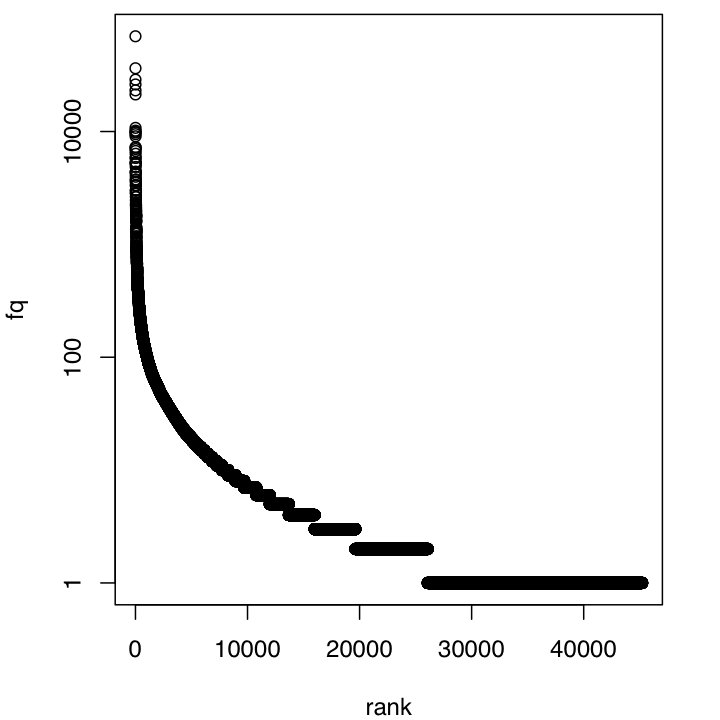
\includegraphics[height=7.5cm]{img/brown-rf}
  \end{center}
\end{frame}

\begin{frame}
  \frametitle{Top and bottom ranks in the Brown corpus}

  \begin{scriptsize}
    \begin{tabular}{|r|r|l||r|r|l|}
      \hline
      \multicolumn{3}{|c||}{\hh{top frequencies}} & \multicolumn{3}{c|}{\hh{bottom frequencies}}\\
      \hline
      \textbf{\textit{r}} & \multicolumn{1}{c|}{\textbf{\textit{f}}} & \textbf{word} & \textbf{rank range} & \multicolumn{1}{c|}{\textbf{\textit{f}}} & \textbf{randomly selected examples}\\
      \hline
      1 & 62642 & the &       7967--\phantom{0}8522 & 10 & recordings, undergone, privileges\\
      2 & 35971 & of &        8523--\phantom{0}9236 & 9 &  Leonard, indulge, creativity\\
      3 & 27831 & and &       9237--10042 & 8 &  unnatural, Lolotte, authenticity\\
      4 & 25608 & to &        10043--11185 & 7 &  diffraction, Augusta, postpone\\
      5 & 21883 & a &         11186--12510 & 6 &  uniformly, throttle, agglutinin\\
      6 & 19474 & in &        12511--14369 & 5 &  Bud, Councilman, immoral\\
      7 & 10292 & that &      14370--16938 & 4 &  verification, gleamed, groin\\
      8 & 10026 & is &        16939--21076 & 3 &  Princes, nonspecifically, Arger\\
      9 & 9887 & was &        21077--28701 & 2 &  blitz, pertinence, arson\\
      10 & 8811 & for &       28702--53076 & 1 &  Salaries, Evensen, parentheses\\
      \hline
    \end{tabular}
  \end{scriptsize}
\end{frame}


\begin{frame}
\frametitle{Frequency spectrum}

  \begin{itemize}
  \item The sample:  \texttt{\textbf{c a a b c c a c d}}
  \item Frequency classes: 1 (\texttt{b}, \texttt{d}), 3 (\texttt{a}), 4 (\texttt{c})
  \item Frequency spectrum:
    \begin{center}
      \begin{tabular}{r|r}
        $m$ & $V_m$\\
        \hline
        1 & 2\\
        3 & 1\\
        4 & 1
      \end{tabular}
    \end{center}
  \end{itemize}
\end{frame}

\begin{frame}
\frametitle{Frequency spectrum of Brown corpus}
   
   \begin{center}
     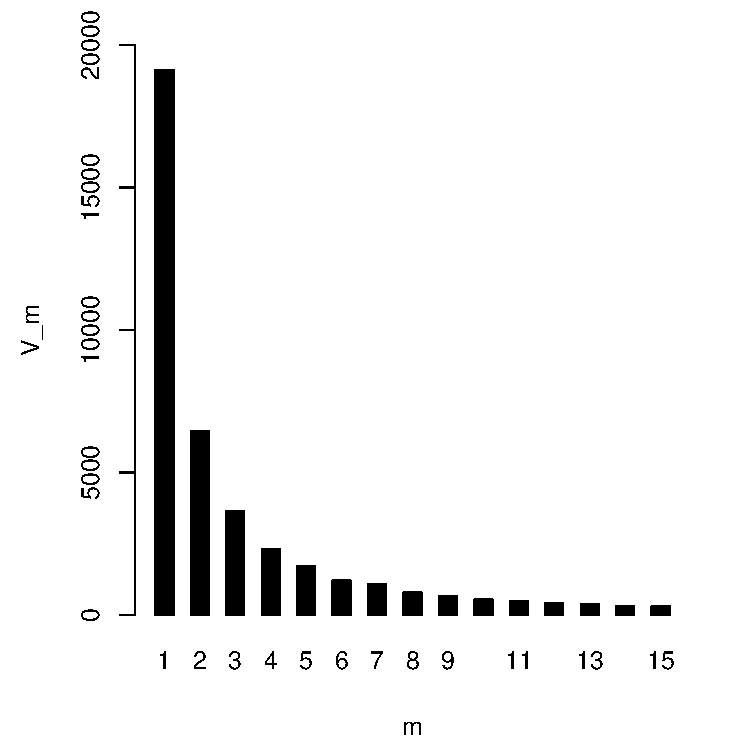
\includegraphics[height=7.5cm]{img/brown-spc}
   \end{center}
 \end{frame}

\begin{frame}
 \frametitle{Vocabulary growth curve}

  \begin{itemize}
  \item<1-> The sample: \texttt{\hh<2->{a} \hh<3->{b b} \hh<4->{c a} \hh<5->{a b a}}
  \item<2-> $N = 1$, $V = 1$, $V_1 = 1$ $\;$ ($V_2 = 0$, \ldots)
  \item<3-> $N = 3$, $V = 2$, $V_1 = 1$ $\;$ ($V_2 = 1$, $V_3 = 0$, \ldots)
  \item<4-> $N = 5$, $V = 3$, $V_1 = 1$ $\;$ ($V_2 = 2$, $V_3 = 0$, \ldots)
  \item<5-> $N = 8$, $V = 3$, $V_1 = 1$ $\;$ ($V_2 = 0$, $V_3 = 1$, $V_4 = 1$, \ldots)
  \end{itemize}
\end{frame}

\begin{frame}
\frametitle{Vocabulary growth curve of Brown corpus}
\framesubtitle{With $V_1$ growth in red (curve smoothed with binomial interpolation)}

  \begin{center}
    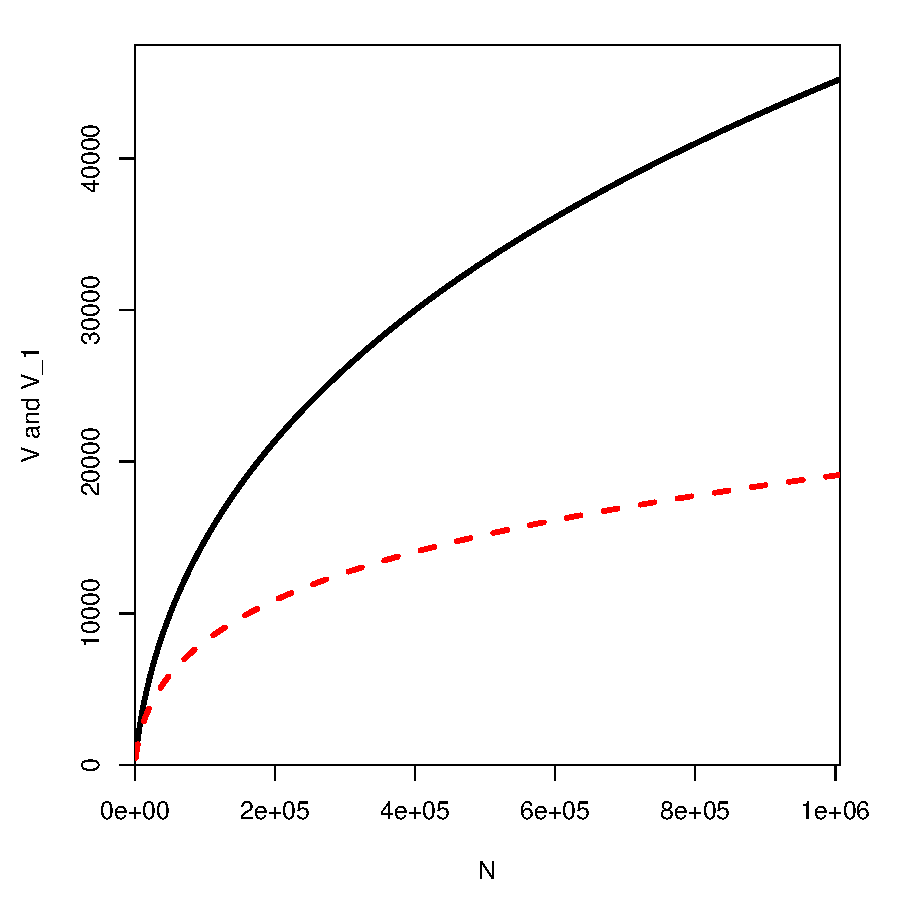
\includegraphics[height=7.5cm]{img/brown-vgc}
  \end{center}
 \end{frame}

\AtBeginSection[]{
  \begin{frame}<beamer:1| handout:0>
    \frametitle{Outline}
    \tableofcontents[current,currentsection]
  \end{frame}}


\AtBeginSubsection[]{
  \begin{frame}<beamer:1| handout:0>
    \frametitle{Outline}
    \tableofcontents[current,currentsubsection]
  \end{frame}}

%%%%%%%%%%%%%%%%%%%%%%%%%%%%%%%%%%%%%%%%%%%%%%%%%%%%%%%%%%%%%%%%%%%%%%%%

\subsection{Typical frequency distribution patterns}

\begin{frame}
  \frametitle{Typical frequency patterns} 
  \framesubtitle{Across text types \& languages}

  \begin{center}
    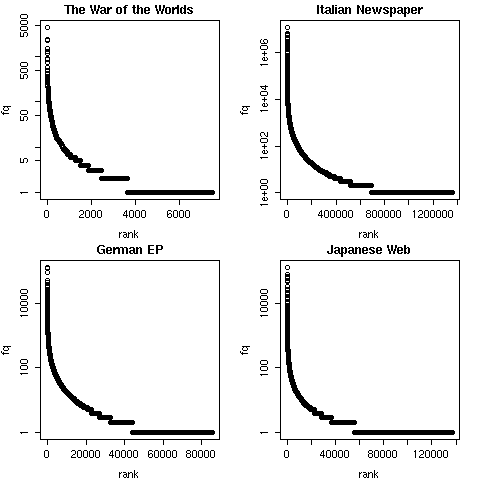
\includegraphics[height=8cm]{img/othercorporarf}
  \end{center}
\end{frame}

\begin{frame}
  \frametitle{Typical frequency patterns} 
  \framesubtitle{The Italian prefix \textcite{ri-} in the \emph{la Repubblica} corpus}

  \begin{center}
    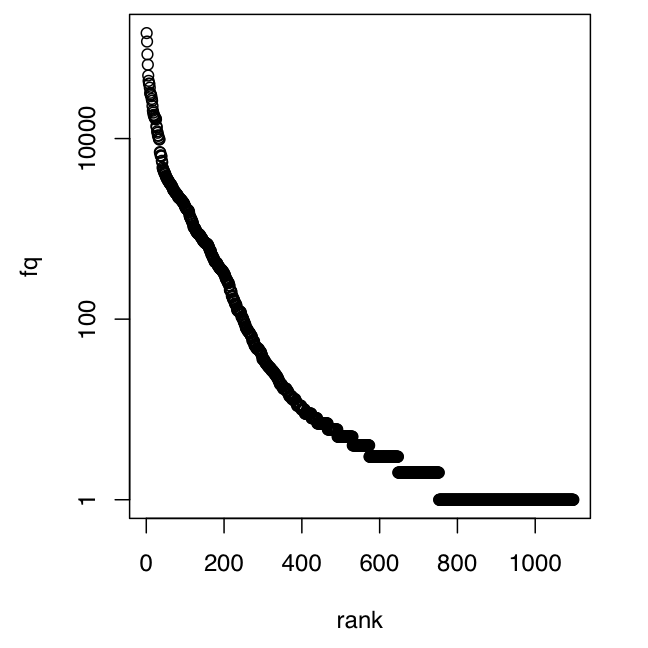
\includegraphics[height=7.5cm]{img/ita-ri-rf}
  \end{center}
\end{frame}

\begin{frame}
  \frametitle{Is there a general law?}

  \begin{itemize}
  \item Language after language, corpus after corpus, linguistic type after
    linguistic type, \ldots\ we observe the same ``few giants, many dwarves'' pattern 
  \item Similarity of plots suggests that relation between rank and
    frequency could be captured by a general law%
    \pause
  \item Nature of this relation becomes clearer if we plot $\log f$ as a
    function of $\log r$ %
    \vspace{-5mm}
    \begin{center}
      \hspace{2cm}
      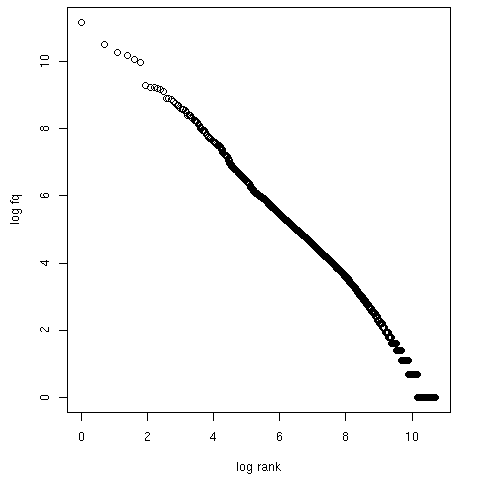
\includegraphics[height=50mm]{img/brown-loglog-rf}
    \end{center}
  \end{itemize}

\end{frame}

%%%%%%%%%%%%%%%%%%%%%%%%%%%%%%%%%%%%%%%%%%%%%%%%%%%%%%%%%%%%%%%%%%%%%%%%

\subsection{Zipf's law}

\begin{frame}
  \frametitle{Zipf's law}

\begin{itemize}
\item Straight line in double-logarithmic space corresponds to
  \h{power law} for original variables
\item This leads to Zipf's (1949, 1965) famous law:
    \[
    f(w)=\frac{C}{r(w)^a}
    \]
    \pause
  \item With $a=1$ and $C=$60,000, Zipf's law predicts that:
    \begin{itemize}
    \item most frequent word occurs 60,000 times
    \item second most frequent word occurs 30,000 times
    \item third most frequent word occurs 20,000 times
    \item and there is a long tail of 80,000 words with frequencies between
      1.5 and 0.5 occurrences(!)
    \end{itemize}
  \end{itemize}

\end{frame}

\begin{frame}
  \frametitle{Zipf's law}\framesubtitle{Logarithmic version}

  \begin{itemize}
  \item Zipf's power law:
    \[
    f(w)=\frac{C}{r(w)^a}
    \]
  \item If we take logarithm of both sides, we obtain:
    \[
    \log f(w)= \log C - a \log r(w)
    \]
  \item Zipf's law predicts that rank / frequency profiles are
    straight lines in double logarithmic space
  \item Best fit $a$ and $C$ can be found with least-squares
    method%
    \pause
  \item Provides intuitive interpretation of $a$ and $C$:
    \begin{itemize}
    \item $a$ is \h{slope} determining how fast log frequency decreases
    \item $\log C$ is \h{intercept}, i.e., predicted log frequency of word
      with rank 1 ($\log$ rank 0) = most frequent word
    \end{itemize}
  \end{itemize}
\end{frame}


\begin{frame}
  \frametitle{Zipf's law}
  \framesubtitle{Fitting the Brown rank/frequency profile}

  \begin{center}
    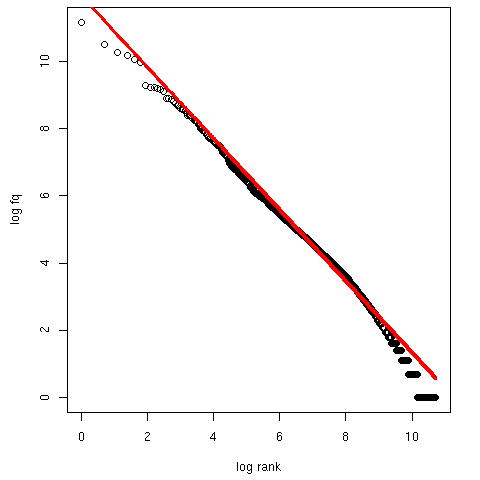
\includegraphics[height=7.5cm]{img/brown-zipf-rf}
  \end{center}
\end{frame}

\begin{frame}
  \frametitle{Zipf-Mandelbrot law}
  \framesubtitle{Mandelbrot 1953}

  \begin{itemize}
    \item Mandelbrot's extra parameter:
    \[
    f(w)=\frac{C}{(r(w) + b)^a}
    \]
  \item Zipf's law is special case with $b=0$
  \item Assuming $a=1$, $C=$60,000, $b=1$:
    \begin{itemize}
    \item For word with rank 1, Zipf's law predicts frequency of
      60,000; Mandelbrot's variation predicts frequency of 30,000
    \item For word with rank 1,000,  Zipf's law predicts frequency of
      60; Mandelbrot's variation predicts frequency of 59.94
    \end{itemize}
  \item[]
  \item Zipf-Mandelbrot law forms basis of statistical LNRE models% 
    \begin{itemize}
    \item ZM law derived mathematically as limiting distribution of
      vocabulary generated by a character-level Markov process
    \end{itemize}
  \end{itemize}
\end{frame}

\begin{frame}
  \frametitle{Zipf-Mandelbrot vs.\ Zipf's law} 
  \framesubtitle{Fitting the Brown rank/frequency profile}

  \begin{center}
    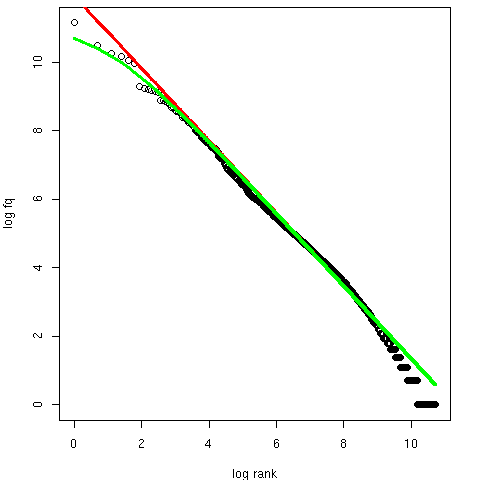
\includegraphics[height=7.5cm]{img/brown-zipf-man-rf}
  \end{center}
\end{frame}

%%%%%%%%%%%%%%%%%%%%%%%%%%%%%%%%%%%%%%%%%%%%%%%%%%%%%%%%%%%%%%%%%%%%%%%%

\subsection{Some applications}

\begin{frame}
  \frametitle{Applications of word frequency distributions}

  \begin{itemize}
  \item Most important application: \h{extrapolation} of vocabulary size and
    frequency spectrum to larger sample sizes
    \begin{itemize}
    \item productivity (in morphology, syntax, \ldots)
    \item lexical richness\\ (in stylometry, language acquisition, clinical linguistics, \ldots)
    \item practical NLP (est.\ proportion of OOV words, typos, \ldots)
    \end{itemize}
  \item[\hand] need method for predicting vocab.\ growth on unseen data
  \item[]\pause
  \item Direct applications of Zipf's law
    \begin{itemize}
    \item population model for Good-Turing smoothing
    \item realistic prior for Bayesian language modelling
    \end{itemize}
  \item[\hand] need model of type probability distribution in the population
  \end{itemize}
\end{frame}

\begin{frame}
  \frametitle{Vocabulary growth: Pronouns vs.\ \textcite{ri-} in Italian}

  \begin{center}
    \begin{tabular}{c||c|c}
      $N$ & $V$ (pron.) & $V$ (\textcite{ri-}) \\
      \hline
       \phantom{0}5000 & 67 & 224 \\
       10000 & 69 & 271 \\
       15000 & 69 & 288 \\
       20000 & 70 & 300 \\
       25000 & 70 & 322 \\
       30000 & 71 & 347 \\
       35000 & 71 & 364 \\
       40000 & 71 & 377 \\
       45000 & 71 & 386 \\
       50000 & 71 & 400 \\
       \ldots & \ldots & \ldots
    \end{tabular}
  \end{center}
\end{frame}

\begin{frame}
  \frametitle{Vocabulary growth: Pronouns vs.\ \textcite{ri-} in Italian}
  \framesubtitle{Vocabulary growth curves}

  \hspace{-1cm}%
  \begin{tabular}{cc}
    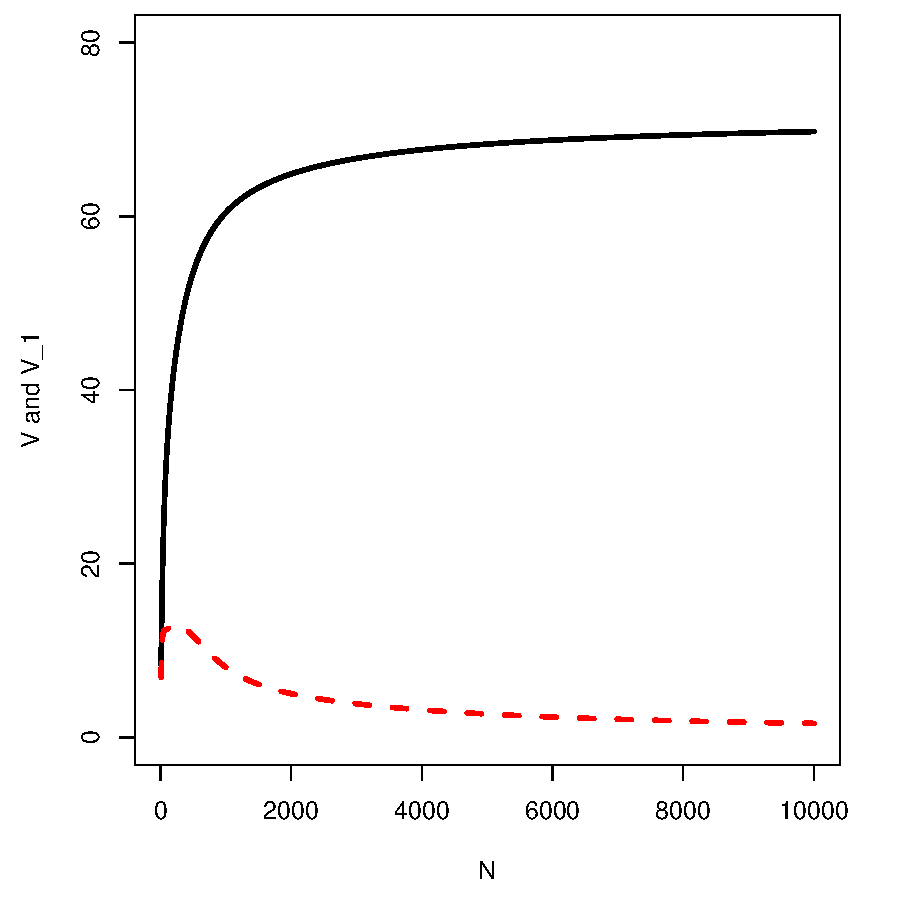
\includegraphics[height=55mm]{img/pro-sub-bin-vgc} &
    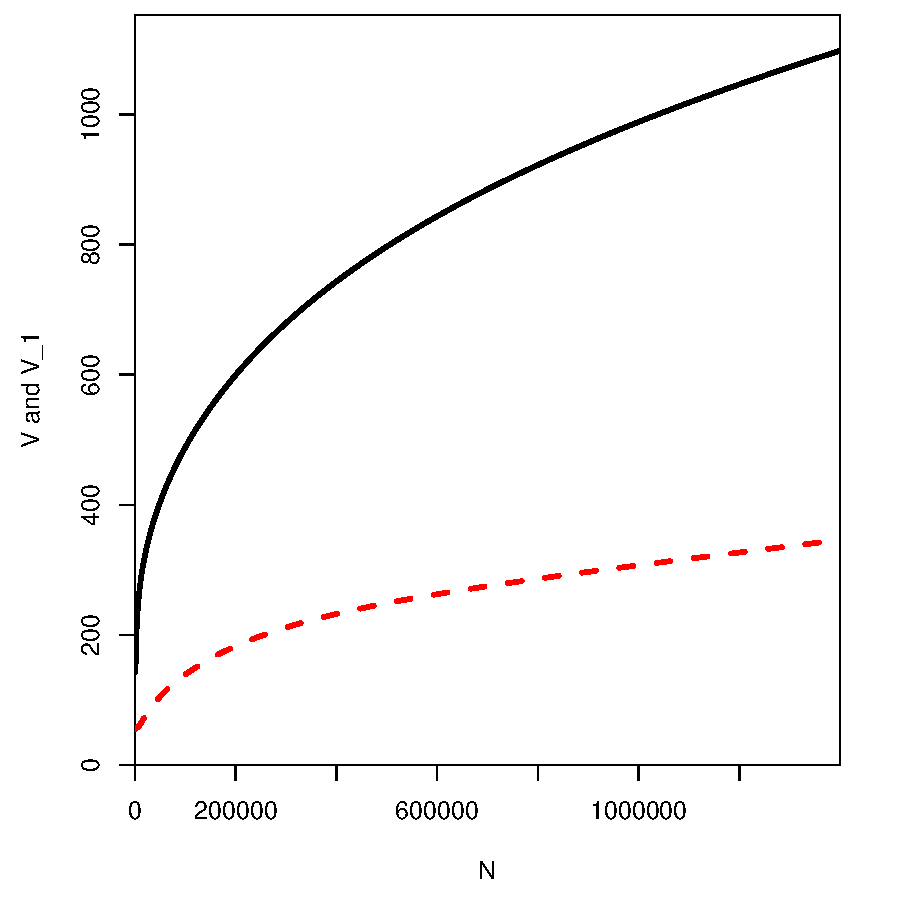
\includegraphics[height=55mm]{img/ita-ri-vgc}
  \end{tabular}
\end{frame}

%%%%%%%%%%%%%%%%%%%%%%%%%%%%%%%%%%%%%%%%%%%%%%%%%%%%%%%%%%%%%%%%%%%%%%%%

\section{Statistical LNRE Models}

\begin{frame}
  \frametitle{LNRE models for word frequency distributions}

  \begin{itemize}
  \item LNRE = large number of rare events (cf.\ Baayen 2001)
  \item Statistics: corpus = random sample from \h{population}
    \begin{itemize}
    \item population characterised by vocabulary of \h{types} $w_k$ with
      occurrence \h{probabilities} $\pi_k$
    \item not interested in specific types \so arrange by decreasing
      probability: $\pi_1\geq \pi_2\geq \pi_3 \geq \cdots$
    \item NB: not necessarily identical to Zipf ranking in sample!
    \end{itemize}
  \item[]\pause
  \item \h{LNRE model} = population model for type probabilities, i.e.\ a
    function $k \mapsto \pi_k$ (with small number of parameters)
    \begin{itemize}
    \item type probabilities $\pi_k$ cannot be estimated reliably from a
      corpus, but parameters of LNRE model can
    \end{itemize}
  \end{itemize}
\end{frame}

\begin{frame}
  \frametitle{Examples of population models}

  \begin{center}
    \begin{tabular}{cc}
      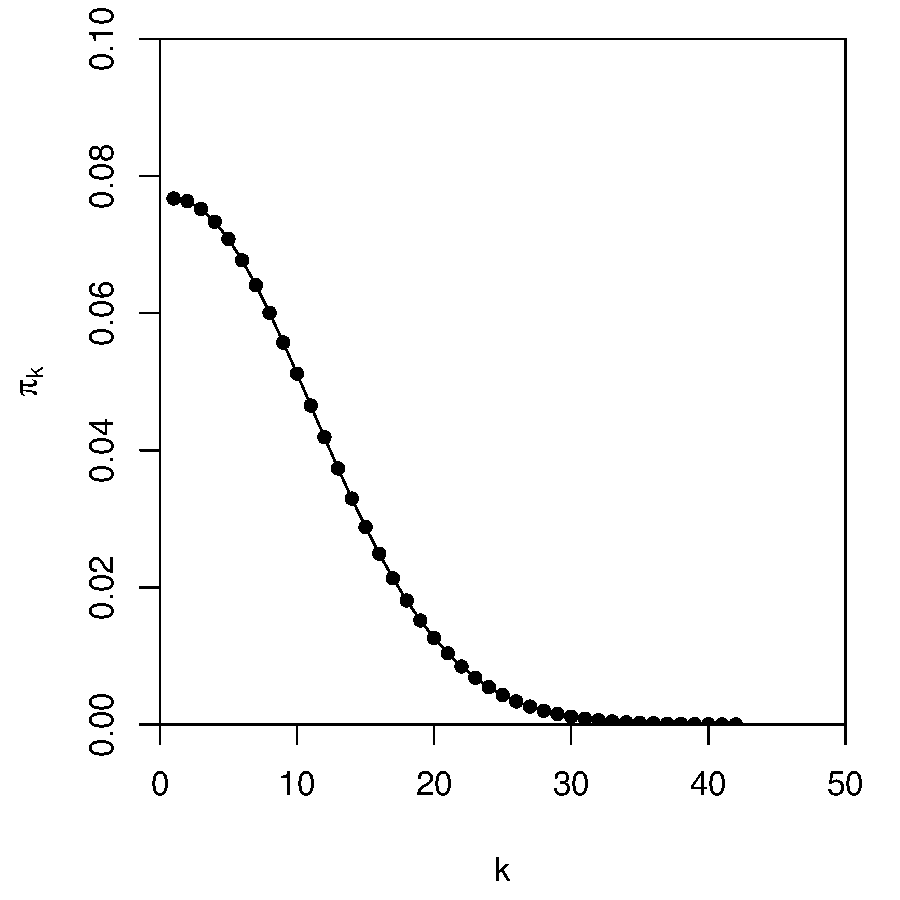
\includegraphics[width=40mm]{img/02-models-normal} &
      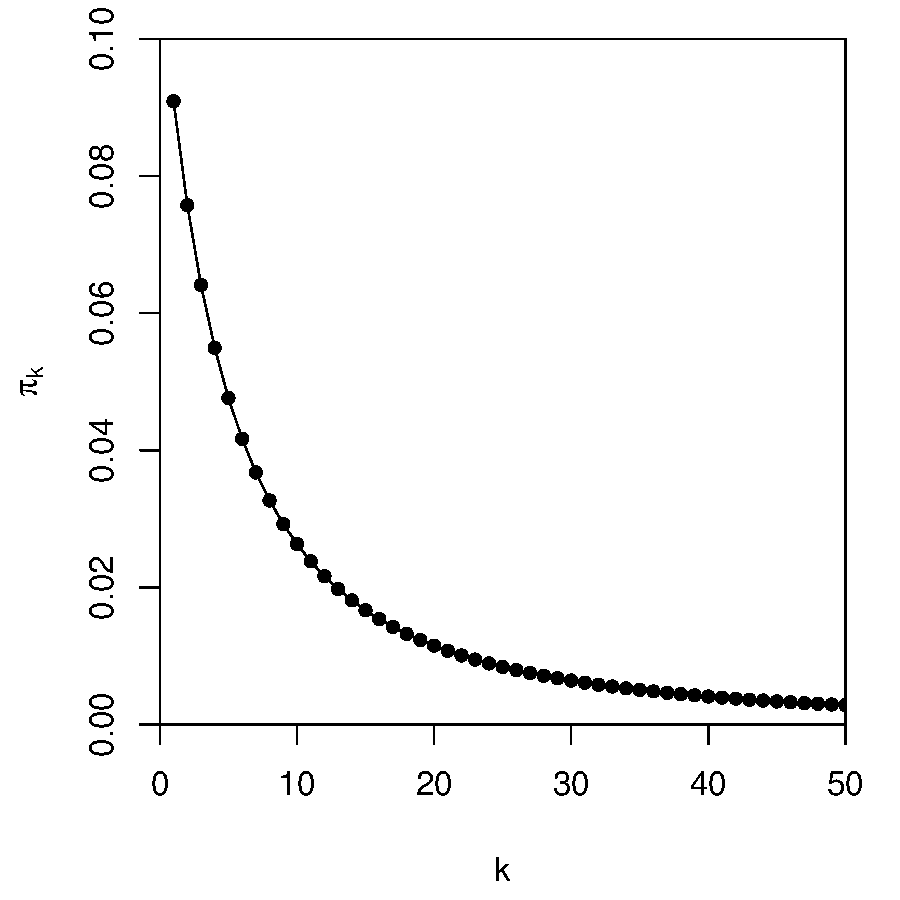
\includegraphics[width=40mm]{img/02-models-zm-1} \\
      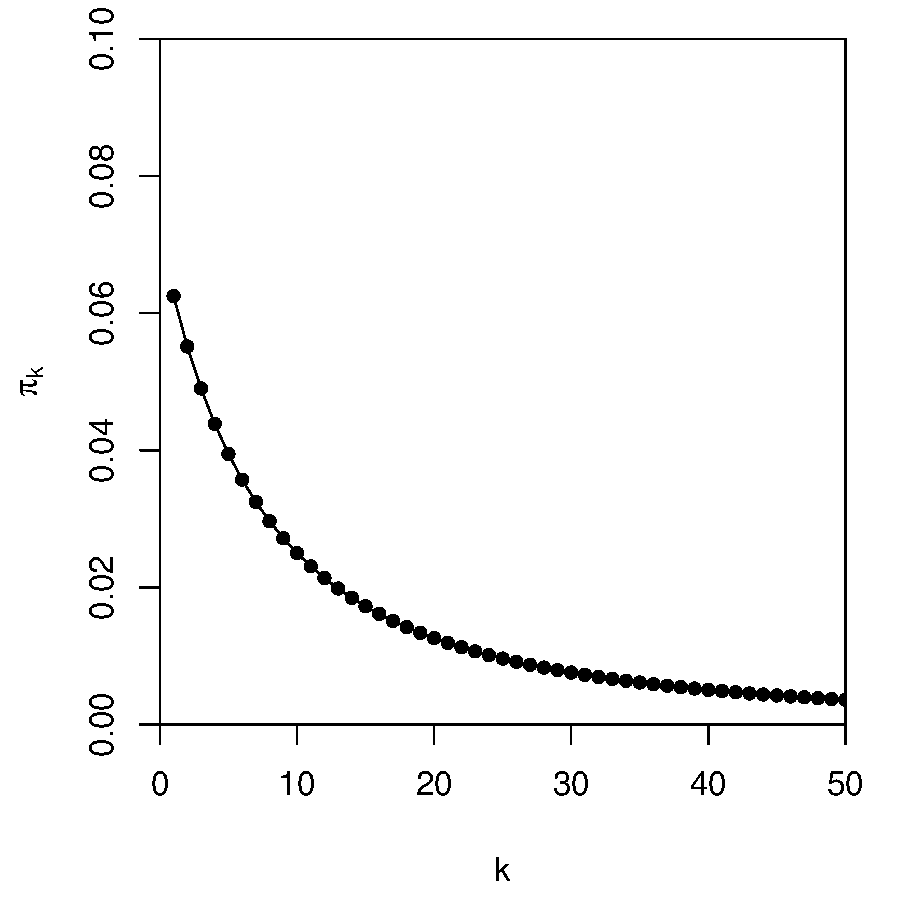
\includegraphics[width=40mm]{img/02-models-zm-3} &
      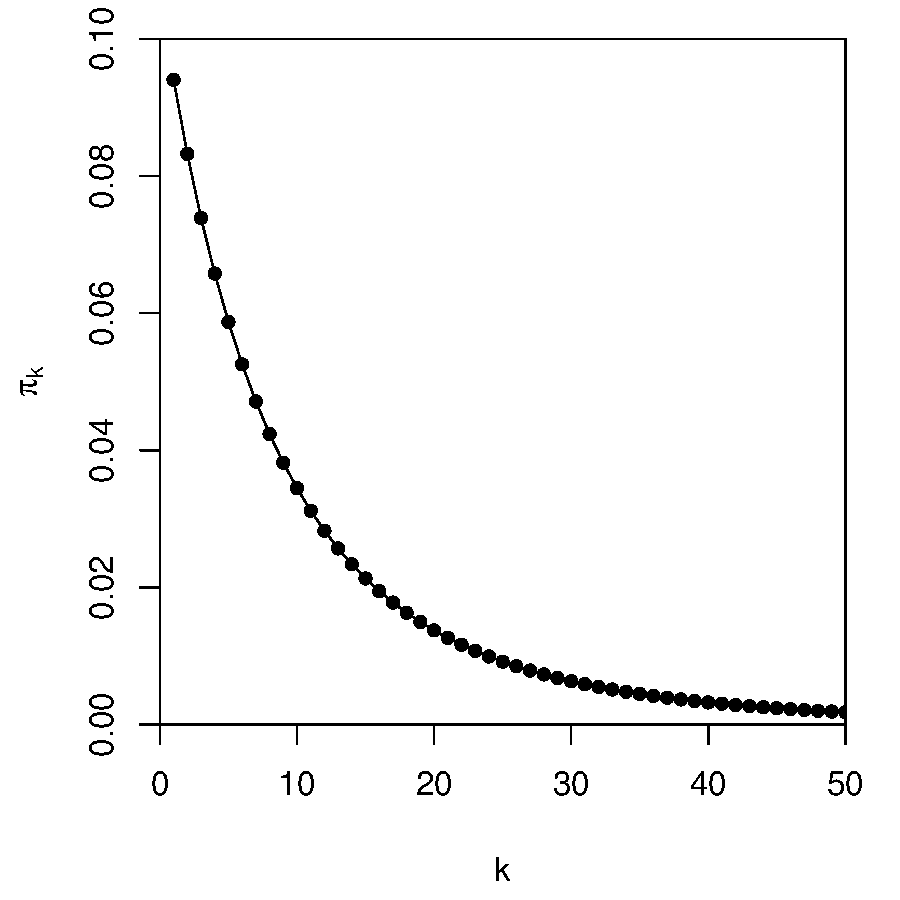
\includegraphics[width=40mm]{img/02-models-zm-2}
    \end{tabular}
  \end{center}
\end{frame}

\begin{frame}
  \frametitle{The Zipf-Mandelbrot law as a population model}

  What is the right family of models for lexical frequency distributions?
  \begin{itemize}
  \item We have already seen that the Zipf-Mandelbrot law captures the
    distribution of observed frequencies very well%
    \pause
  \item Re-phrase the law for type probabilities:
    \[ \pi_k := \frac{C}{(k + b) ^ a} \]
  \item Two free parameters: $a > 1$ and $b \geq 0$
  \item $C$ is not a parameter but a normalization constant,\\
    needed to ensure that $\sum_k \pi_k = 1$
  \item this is the \h{Zipf-Mandelbrot} population model
  \end{itemize}
\end{frame}

%%%%%%%%%%%%%%%%%%%%%%%%%%%%%%%%%%%%%%%%%%%%%%%%%%%%%%%%%%%%%%%%%%%%%%%%

\subsection{ZM \& fZM}

\begin{frame}
  \frametitle{The parameters of the Zipf-Mandelbrot model}

  \begin{center}
    \begin{tabular}{cc}
      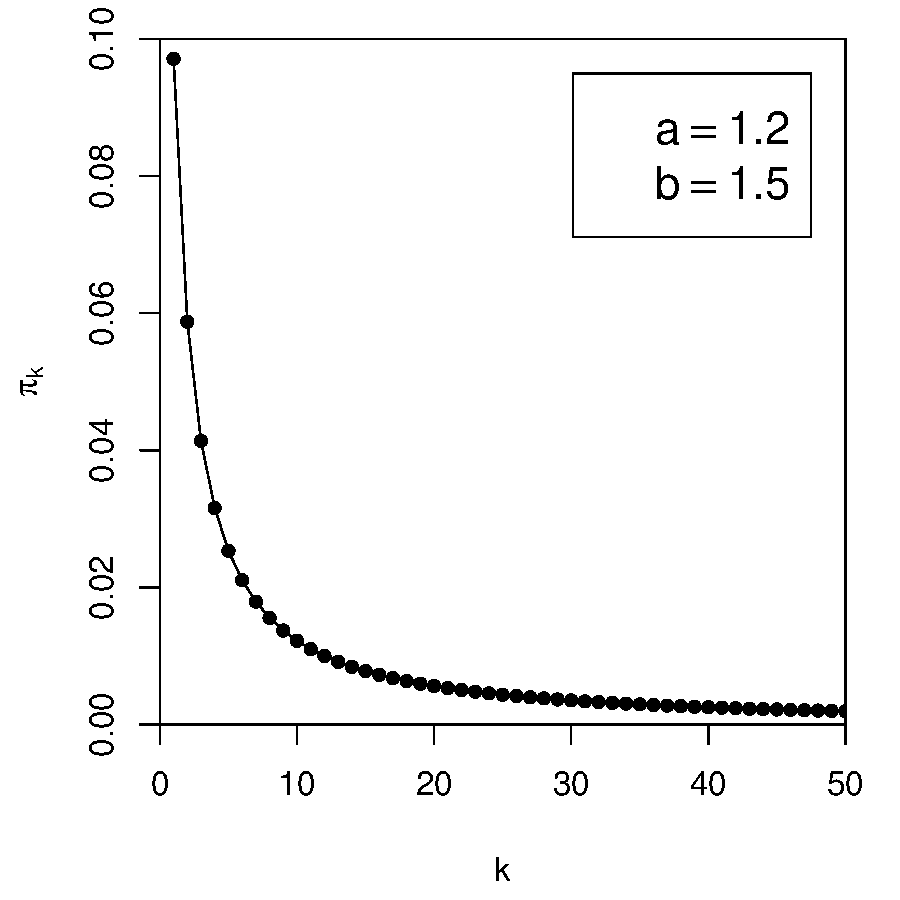
\includegraphics[width=40mm]{img/02-models-zm-param-4} &
      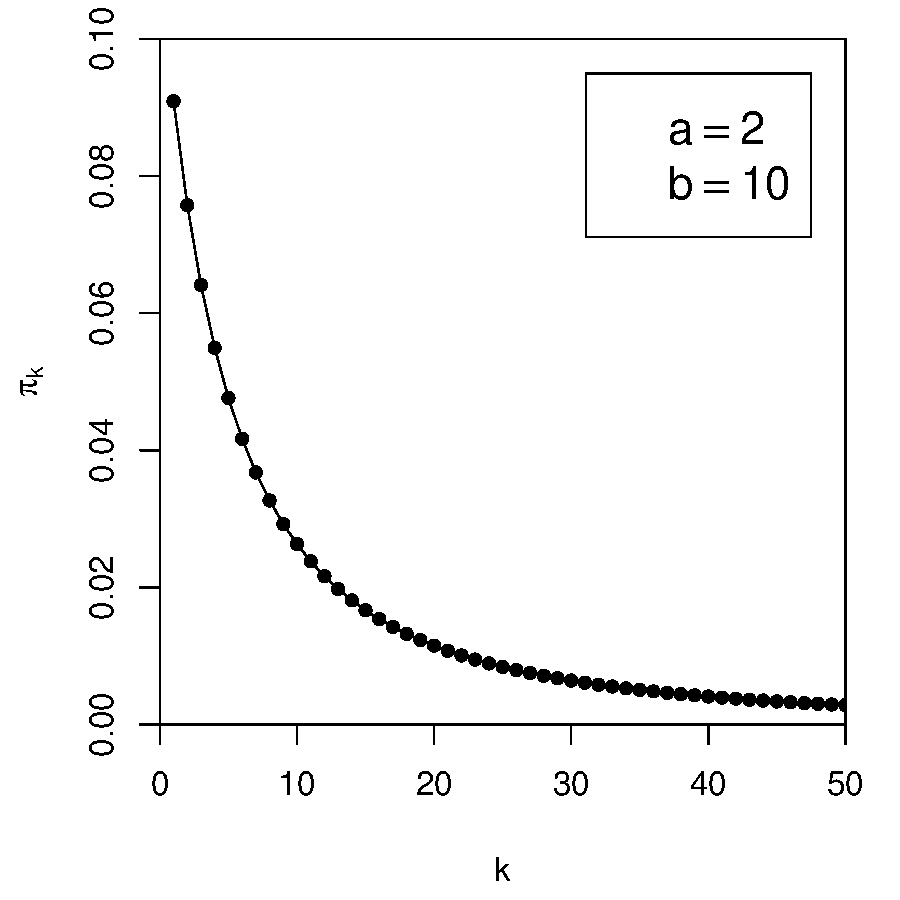
\includegraphics[width=40mm]{img/02-models-zm-param-1} \\
      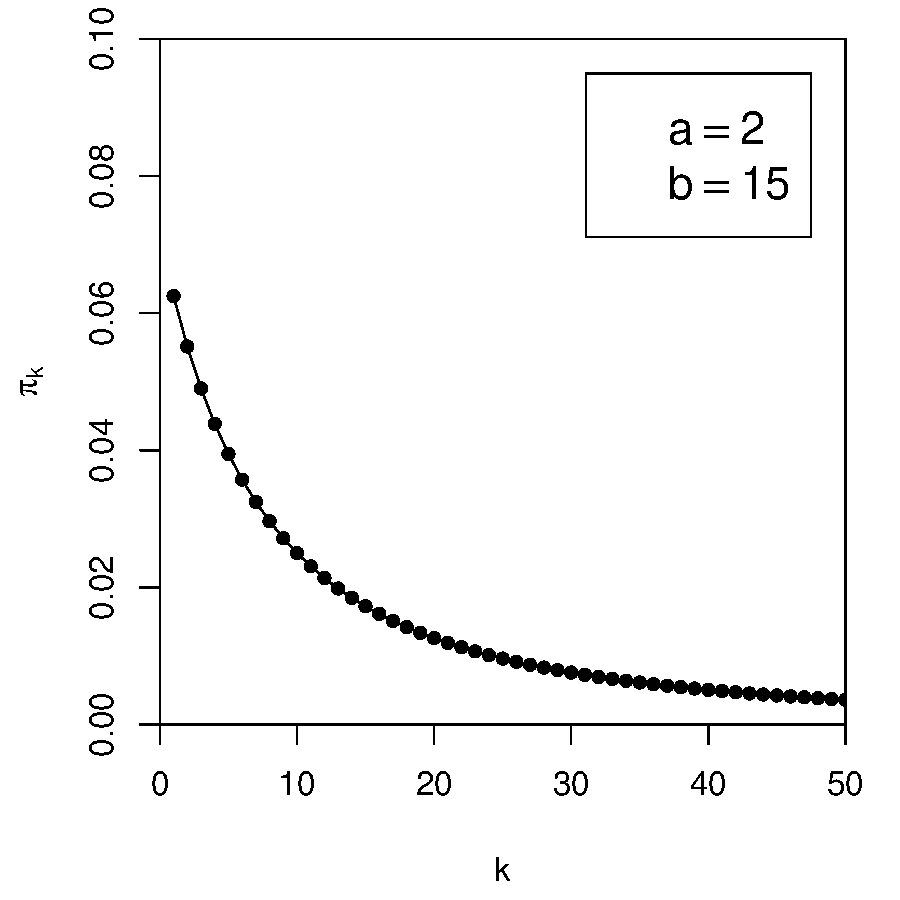
\includegraphics[width=40mm]{img/02-models-zm-param-3} &
      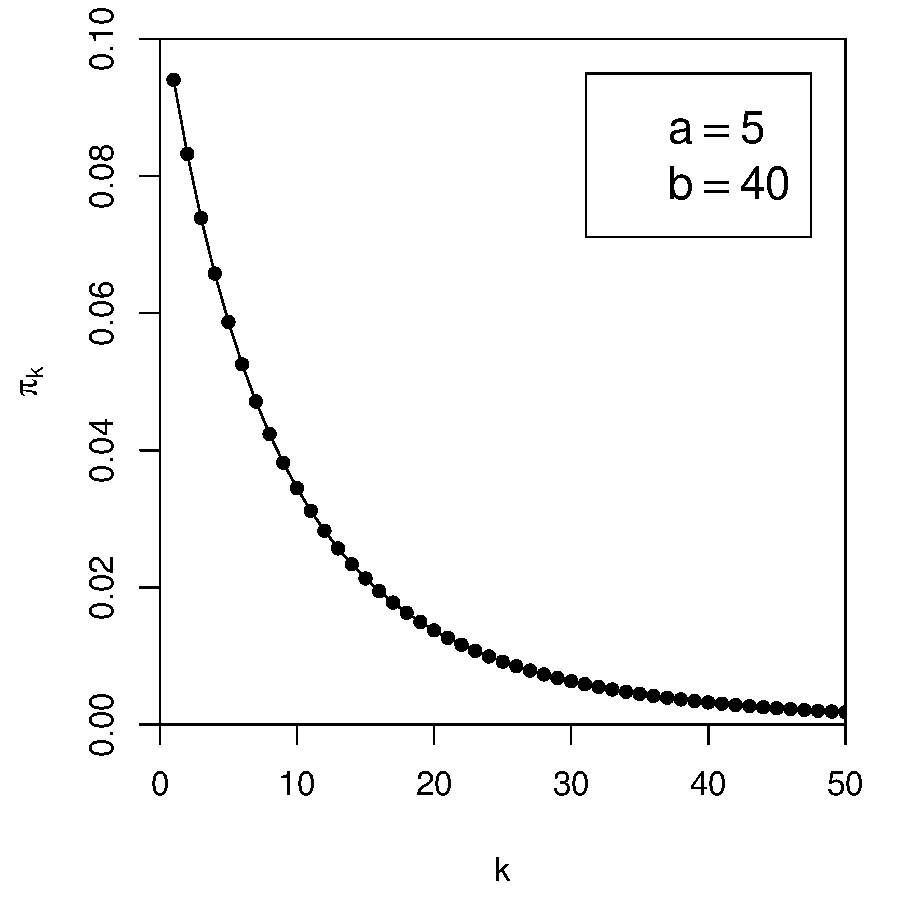
\includegraphics[width=40mm]{img/02-models-zm-param-2}
    \end{tabular}
  \end{center}
\end{frame}

\begin{frame}
  \frametitle{The parameters of the Zipf-Mandelbrot model}

  \begin{center}
    \begin{tabular}{cc}
      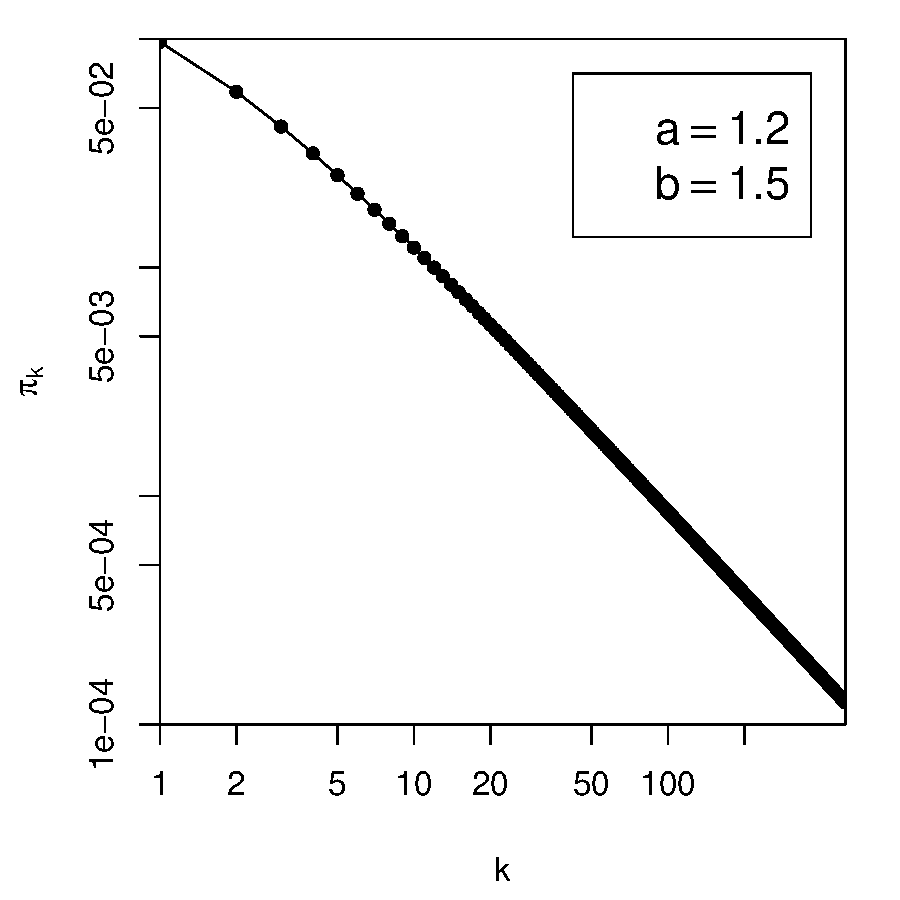
\includegraphics[width=40mm]{img/02-models-zm-log-4} &
      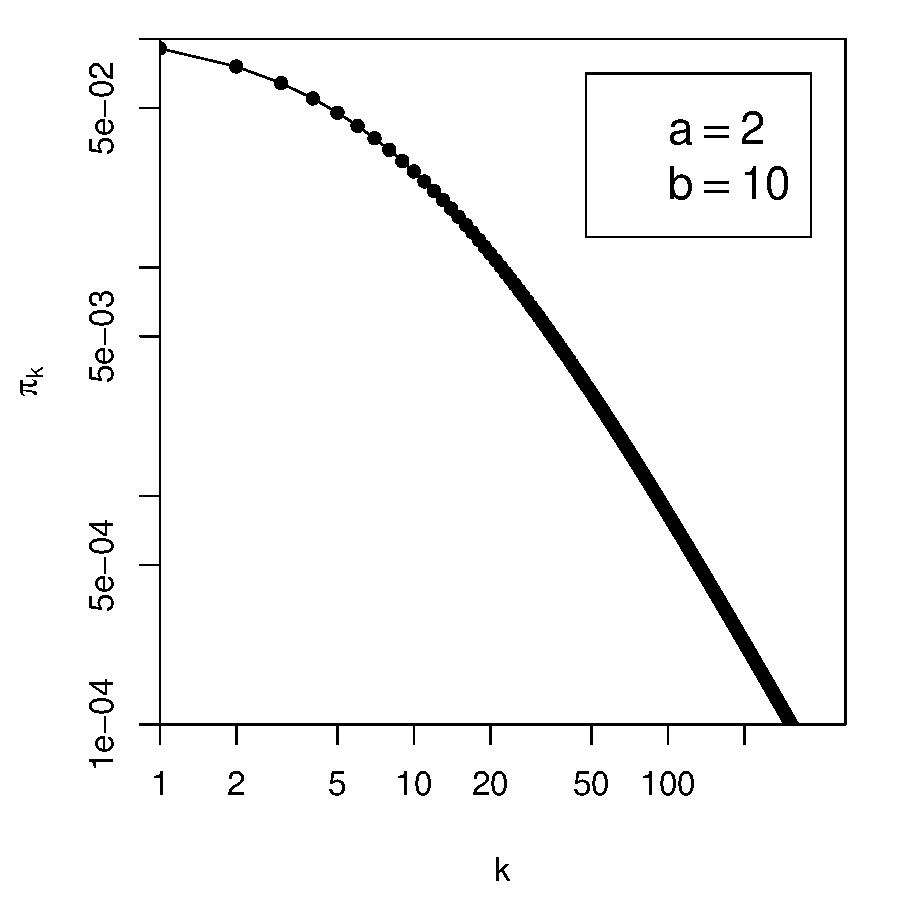
\includegraphics[width=40mm]{img/02-models-zm-log-1} \\
      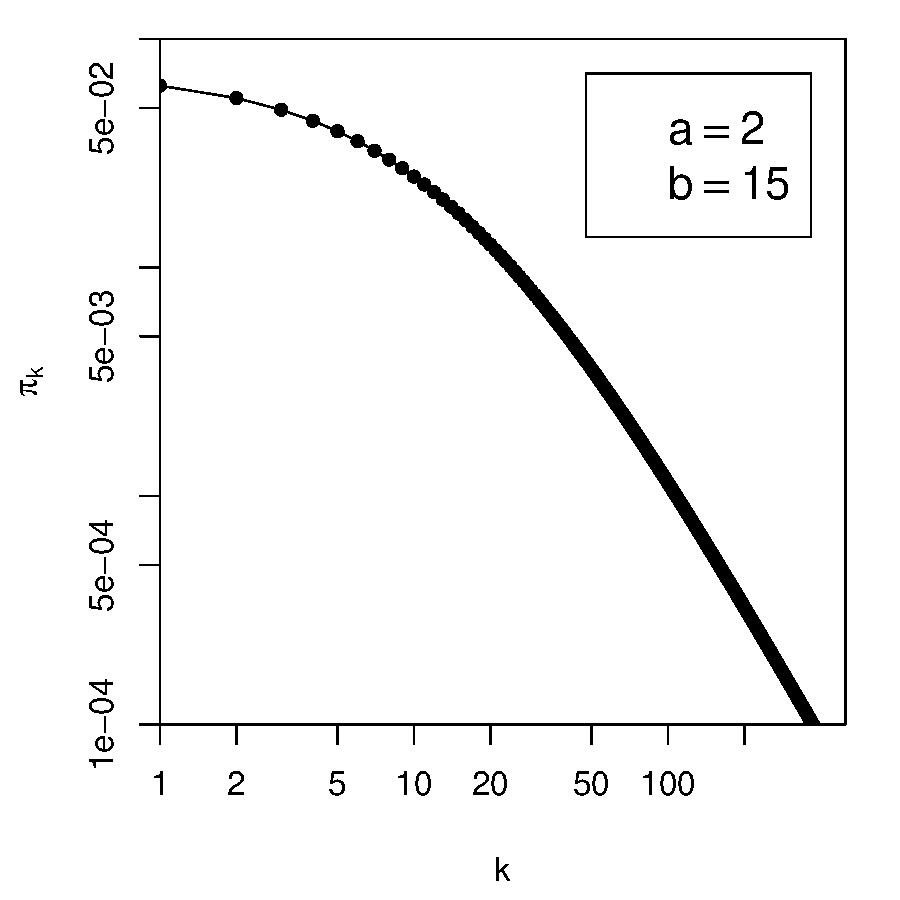
\includegraphics[width=40mm]{img/02-models-zm-log-3} &
      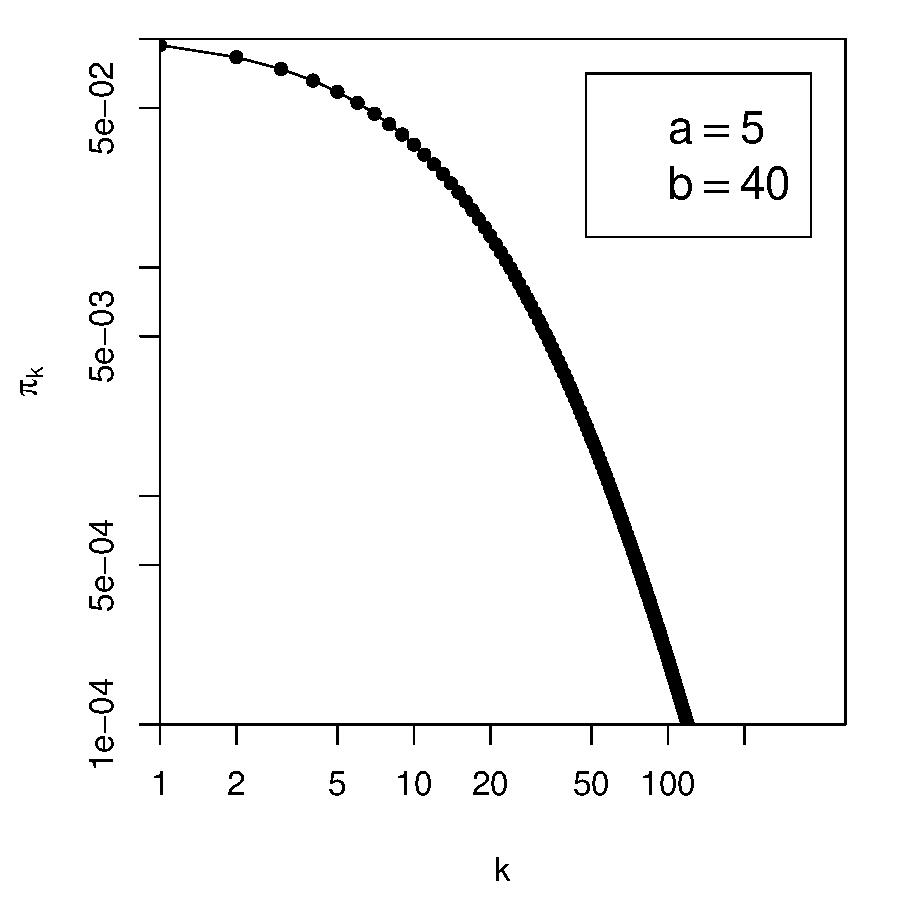
\includegraphics[width=40mm]{img/02-models-zm-log-2}
    \end{tabular}
  \end{center}
\end{frame}


\begin{frame}
  \frametitle{The finite Zipf-Mandelbrot model}

  \begin{itemize}
  \item Zipf-Mandelbrot population model characterizes an \emph{infinite} type
    population: there is no upper bound on $k$, and the type probabilities
    $\pi_k$ can become arbitrarily small
  \item $\pi = 10^{-6}$ (once every million words), $\pi = 10^{-9}$ (once
    every billion words), $\pi = 10^{-12}$ (once on the entire Internet), $\pi
    = 10^{-100}$ (once in the universe?)%
    \pause
  \item Alternative: finite (but often very large) number\\
    of types in the population
  \item We call this the \h{population vocabulary size} $S$\\
    (and write $S = \infty$ for an infinite type population)
  \end{itemize}
\end{frame}

\begin{frame}
  \frametitle{The finite Zipf-Mandelbrot model}

  \begin{itemize}
  \item The \h{finite Zipf-Mandelbrot} model simply stops after the first $S$
    types ($w_1, \ldots, w_S$)
  \item $S$ becomes a new parameter of the model\\
    $\to$ the finite Zipf-Mandelbrot model has 3 parameters
  \end{itemize}

  Abbreviations: 
  \begin{itemize}
  \item \h{ZM} for Zipf-Mandelbrot model
  \item \h{fZM} for finite Zipf-Mandelbrot model
  \end{itemize}
\end{frame}

%%%%%%%%%%%%%%%%%%%%%%%%%%%%%%%%%%%%%%%%%%%%%%%%%%%%%%%%%%%%%%%%%%%%%%%%

\subsection{Sampling from a LNRE model}

\begin{frame}
  \frametitle{Sampling from a population model}

  Assume we believe that the population we are interested in can be described
  by a Zipf-Mandelbrot model: % with parameters $a=3$ and $b=50$
  \begin{center}
    \begin{tabular}{cc}
      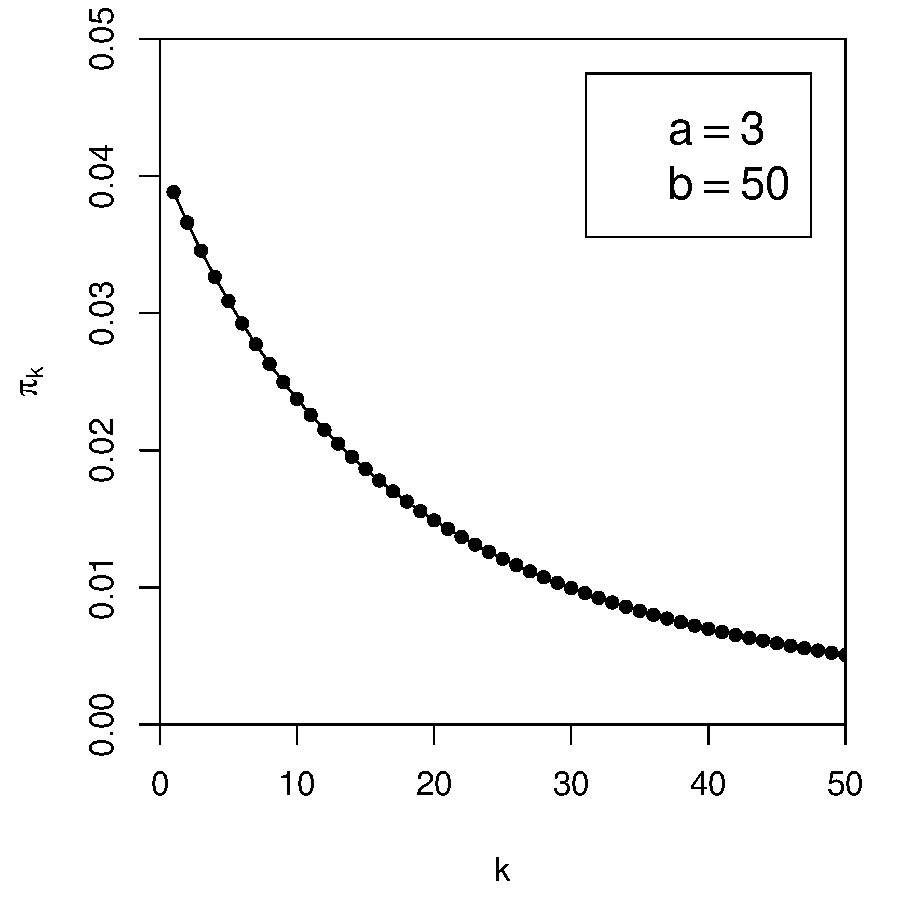
\includegraphics[width=30mm]{img/02-samples-zm-model} &
      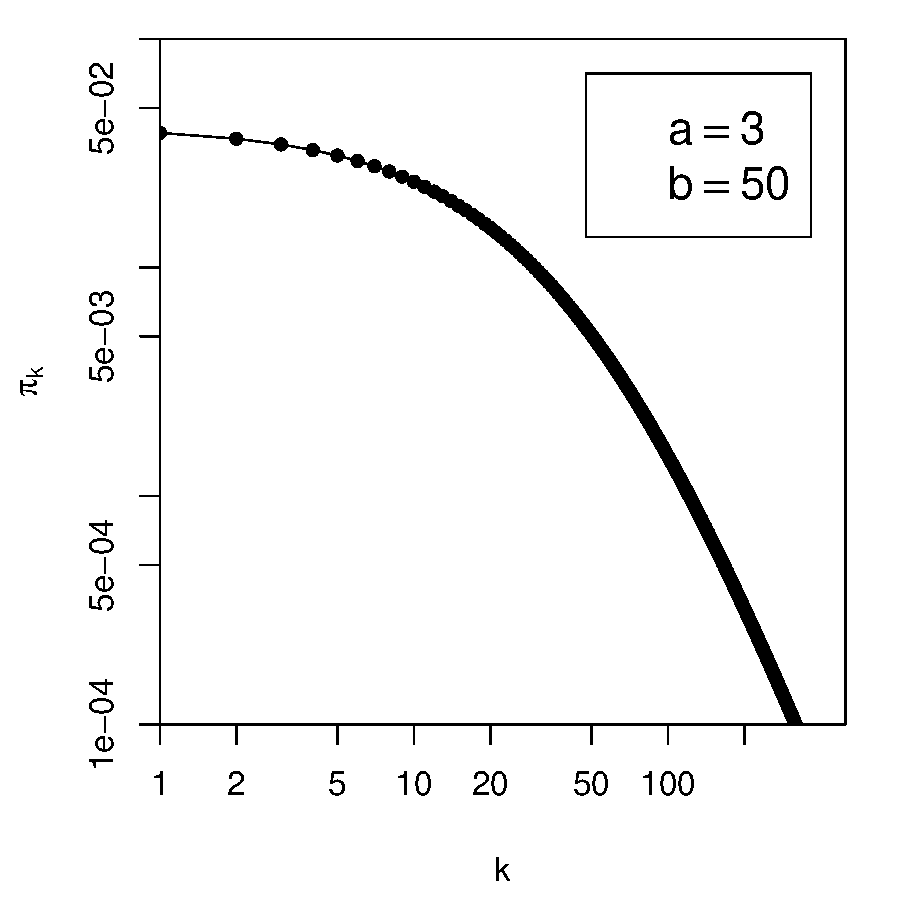
\includegraphics[width=30mm]{img/02-samples-zm-model-log} 
    \end{tabular}
  \end{center}
  
  Use computer simulation to sample from this model:
  \begin{itemize}
  \item Draw $N$ tokens from the population such that in\\
    each step, type $w_k$ has probability $\pi_k$ to be picked
  \item This allows us to make predictions for samples (= corpora) of
    arbitrary size $N$ \so extrapolation
  \end{itemize}
\end{frame}


\begin{frame}
  \frametitle{Sampling from a population model}

  \begin{center}
    \footnotesize
    \begin{tabular}{r *{9}{ @{\hspace{1mm}}r } r}
      \hh{\#1:} &   1 &  42 &  34 &  23 & 108 &  18 &  48 &  18 &   1 & \ldots \\ 
       \pause
      & time & order & room & school & town & course & area & course & time & \ldots \\
       \pause\\
      \hh{\#2:} & 286 &  28 &  23 &  36 &   3 &   4 &   7 &   4 &   8 & \ldots \\ 
       \pause\\
      \hh{\#3:} &   2 &  11 & 105 &  21 &  11 &  17 &  17 &   1 &  16 & \ldots \\ 
       \pause\\
      \hh{\#4:} &  44 &   3 & 110 &  34 & 223 &   2 &  25 &  20 &  28 & \ldots \\ 
       \\
      \hh{\#5:} &  24 &  81 &  54 &  11 &   8 &  61 &   1 &  31 &  35 & \ldots \\ 
      \\
      \hh{\#6:} &   3 &  65 &   9 & 165 &   5 &  42 &  16 &  20 &   7 & \ldots \\ 
      \\
      \hh{\#7:} &  10 &  21 &  11 &  60 & 164 &  54 &  18 &  16 & 203 & \ldots \\ 
      \\
      \hh{\#8:} &  11 &   7 & 147 &   5 &  24 &  19 &  15 &  85 &  37 & \ldots \\
      \\
      \vdots & \vdots & \vdots & \vdots & \vdots & \vdots & \vdots & \vdots & \vdots & \vdots
    \end{tabular}
  \end{center}
\end{frame}

\begin{frame}
  \frametitle{Samples: type frequency list \& spectrum}

  \begin{center}
    \begin{tabular}[t]{r | rr}
      rank $r$ & $f_r$ & type $k$ \\
      \hline
       1 & 37 &  6 \\
       2 & 36 &  1 \\
       3 & 33 &  3 \\
       4 & 31 &  7 \\
       5 & 31 & 10 \\
       6 & 30 &  5 \\
       7 & 28 & 12 \\
       8 & 27 &  2 \\
       9 & 24 &  4 \\
      10 & 24 & 16 \\
      11 & 23 &  8 \\
      12 & 22 & 14 \\
      \vdots & \vdots & \vdots
    \end{tabular}
    \hspace{2cm}
    \begin{tabular}[t]{r | r}
      $m$ & $V_m$ \\
      \hline
       1 & 83 \\
       2 & 22 \\
       3 & 20 \\
       4 & 12 \\
       5 & 10 \\
       6 &  5 \\
       7 &  5 \\
       8 &  3 \\
       9 &  3 \\
      10 &  3 \\
      \vdots & \vdots \\
      \multicolumn{2}{c}{} \\
      \multicolumn{2}{c}{\hh{sample \#1}}
    \end{tabular}
  \end{center}
\end{frame}

\begin{frame}
  \frametitle{Samples: type frequency list \& spectrum}

  \begin{center}
    \begin{tabular}[t]{r | rr}
      rank $r$ & $f_r$ & type $k$ \\
      \hline
       1 & 39 &  2 \\
       2 & 34 &  3 \\
       3 & 30 &  5 \\
       4 & 29 & 10 \\
       5 & 28 &  8 \\
       6 & 26 &  1 \\
       7 & 25 & 13 \\
       8 & 24 &  7 \\
       9 & 23 &  6 \\
      10 & 23 & 11 \\
      11 & 20 &  4 \\
      12 & 19 & 17 \\
      \vdots & \vdots & \vdots
    \end{tabular}
    \hspace{2cm}
    \begin{tabular}[t]{r | r}
      $m$ & $V_m$ \\
      \hline
       1 & 76 \\
       2 & 27 \\
       3 & 17 \\
       4 & 10 \\
       5 &  6 \\
       6 &  5 \\
       7 &  7 \\
       8 &  3 \\
      10 &  4 \\
      11 &  2 \\
      \vdots & \vdots \\
      \multicolumn{2}{c}{} \\
      \multicolumn{2}{c}{\hh{sample \#2}}
    \end{tabular}
  \end{center}
\end{frame}

\begin{frame}
  \frametitle{Random variation in type-frequency lists}

  \begin{tabular}{ccc}
    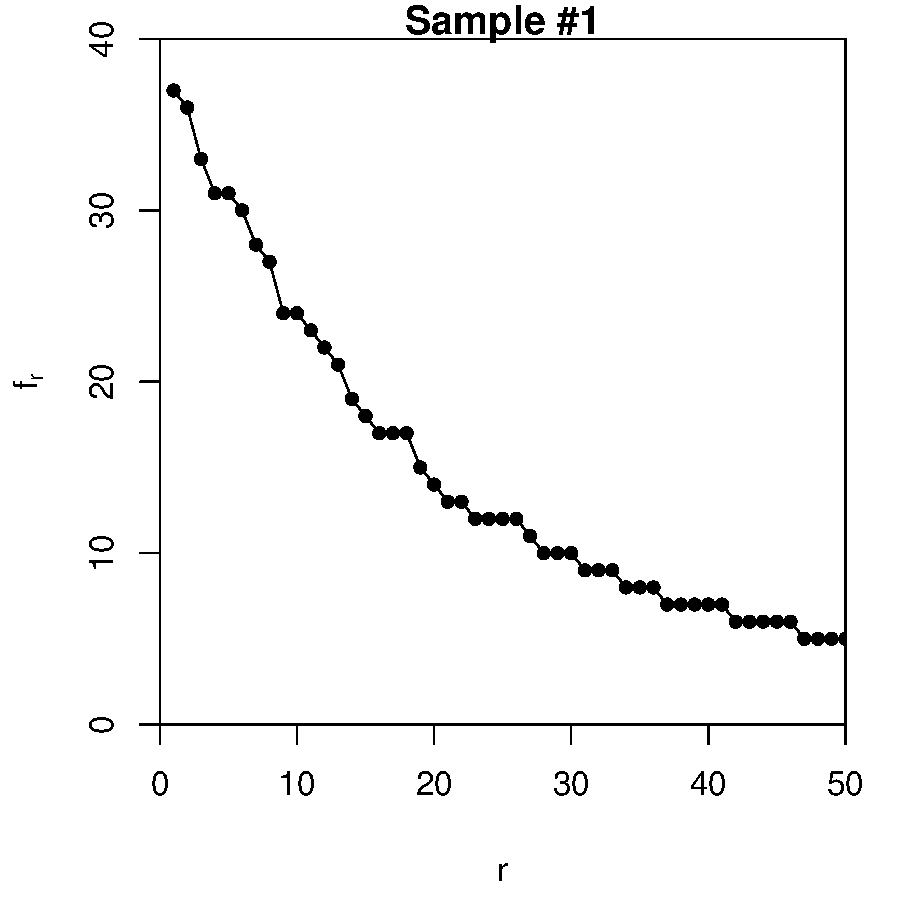
\includegraphics[width=40mm]{img/02-samples-tfl-r-1} &
    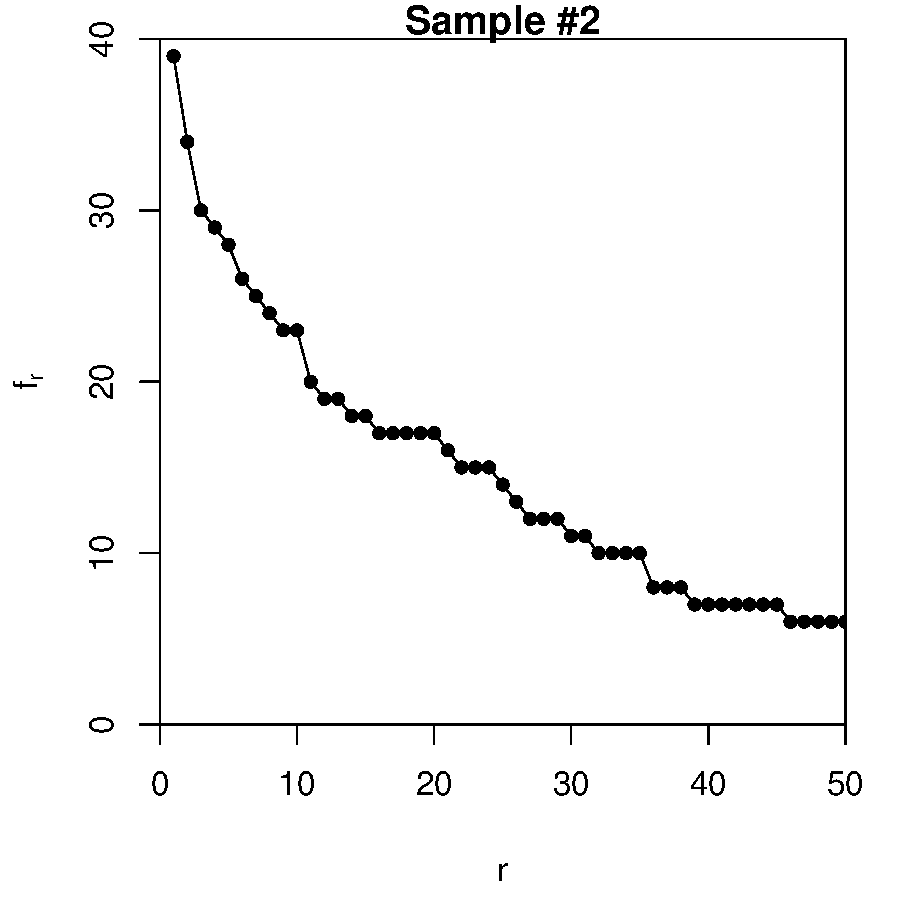
\includegraphics[width=40mm]{img/02-samples-tfl-r-2} &
    \raisebox{2cm}{$r\leftrightarrow f_r$} \\
    
    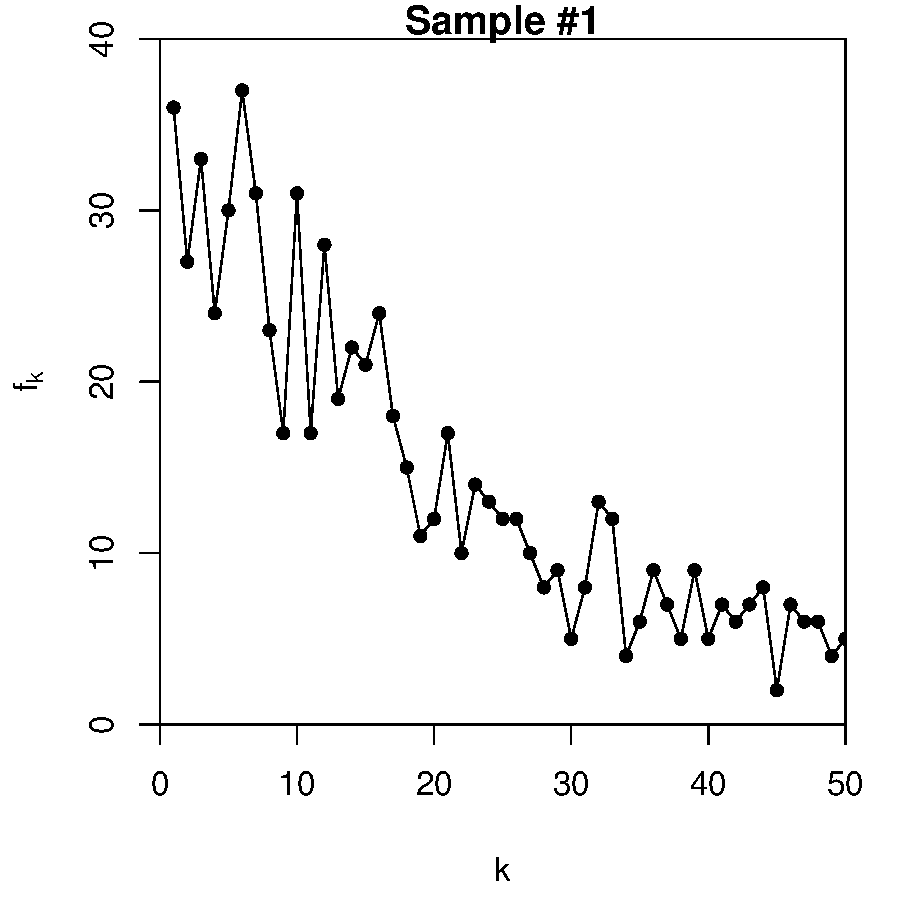
\includegraphics[width=40mm]{img/02-samples-tfl-k-1} &
    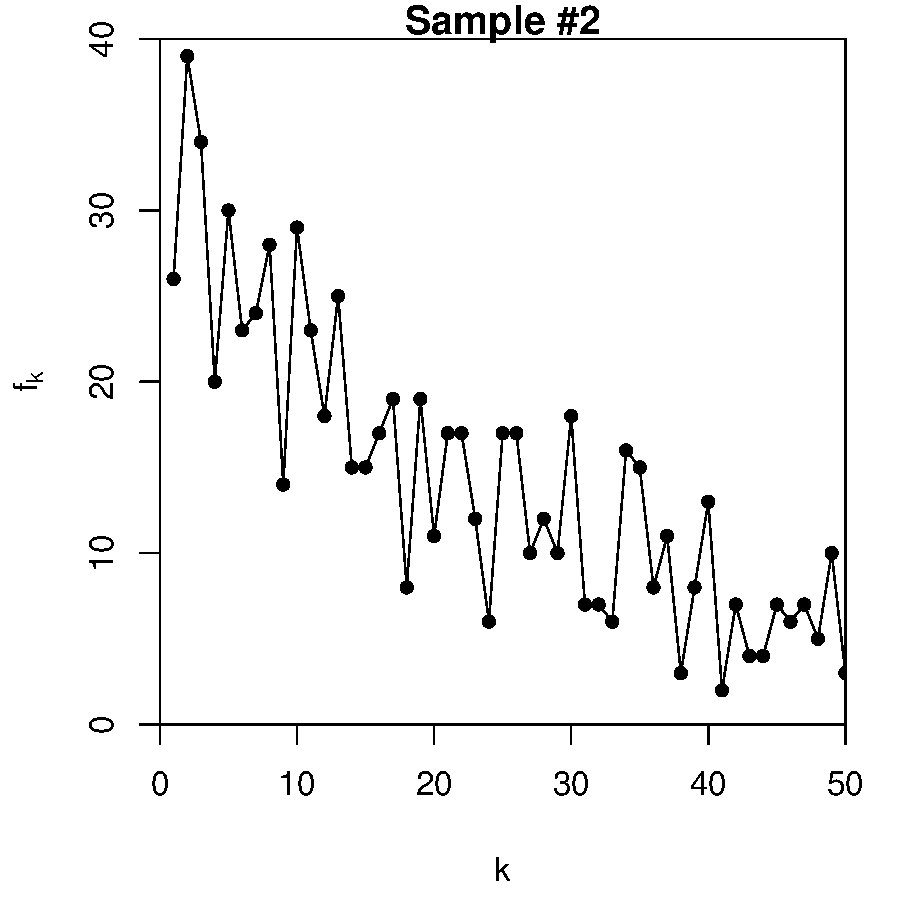
\includegraphics[width=40mm]{img/02-samples-tfl-k-2} &
    \raisebox{2cm}{$k\leftrightarrow f_k$} 
  \end{tabular}
\end{frame}

\begin{frame}
  \frametitle{Random variation: frequency spectrum}

  \begin{center}
    \begin{tabular}{cc}
      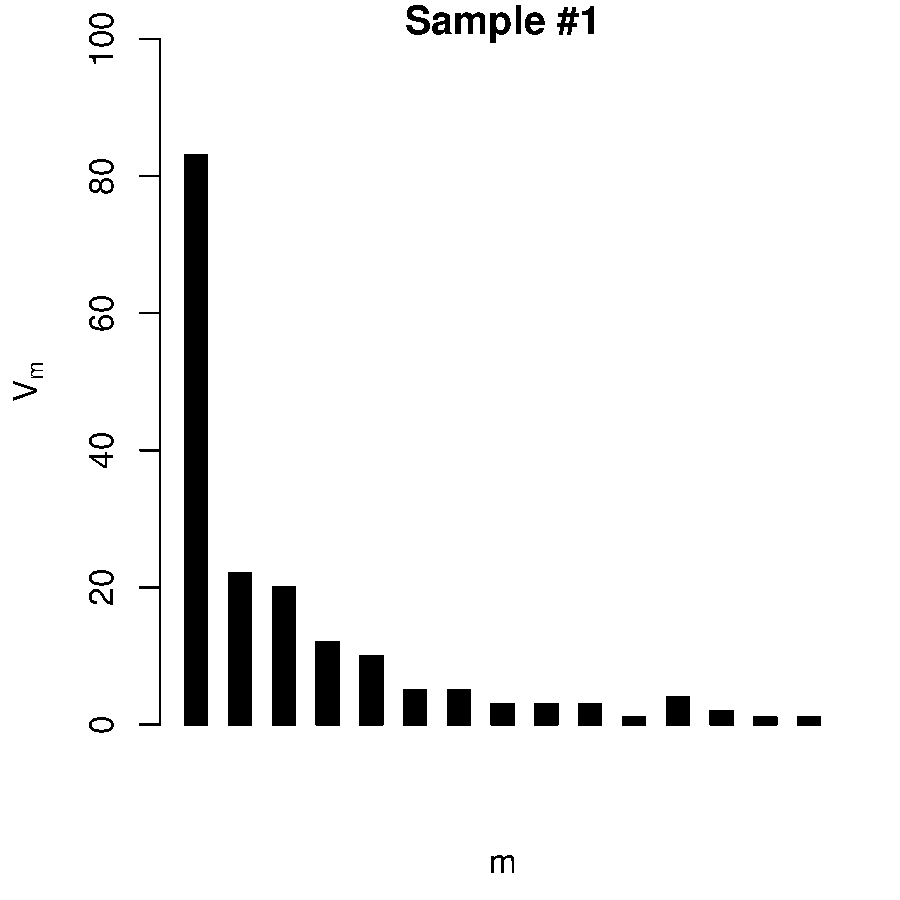
\includegraphics[width=40mm]{img/02-samples-spc-1} &
      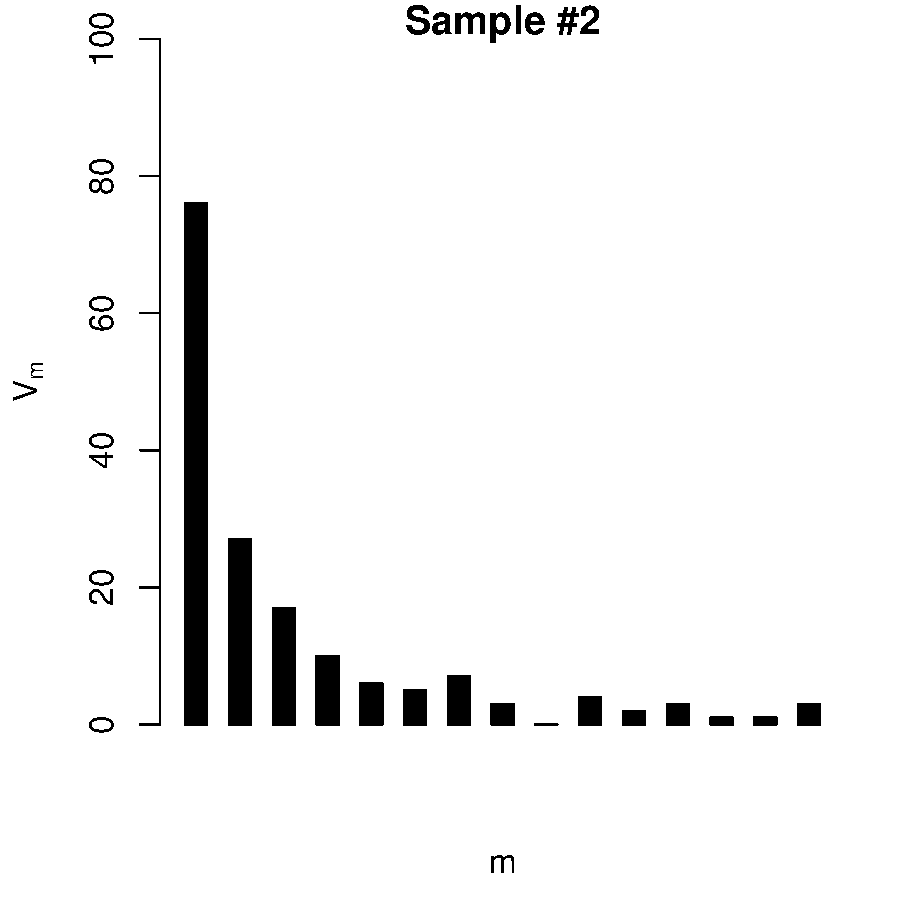
\includegraphics[width=40mm]{img/02-samples-spc-2} \\
      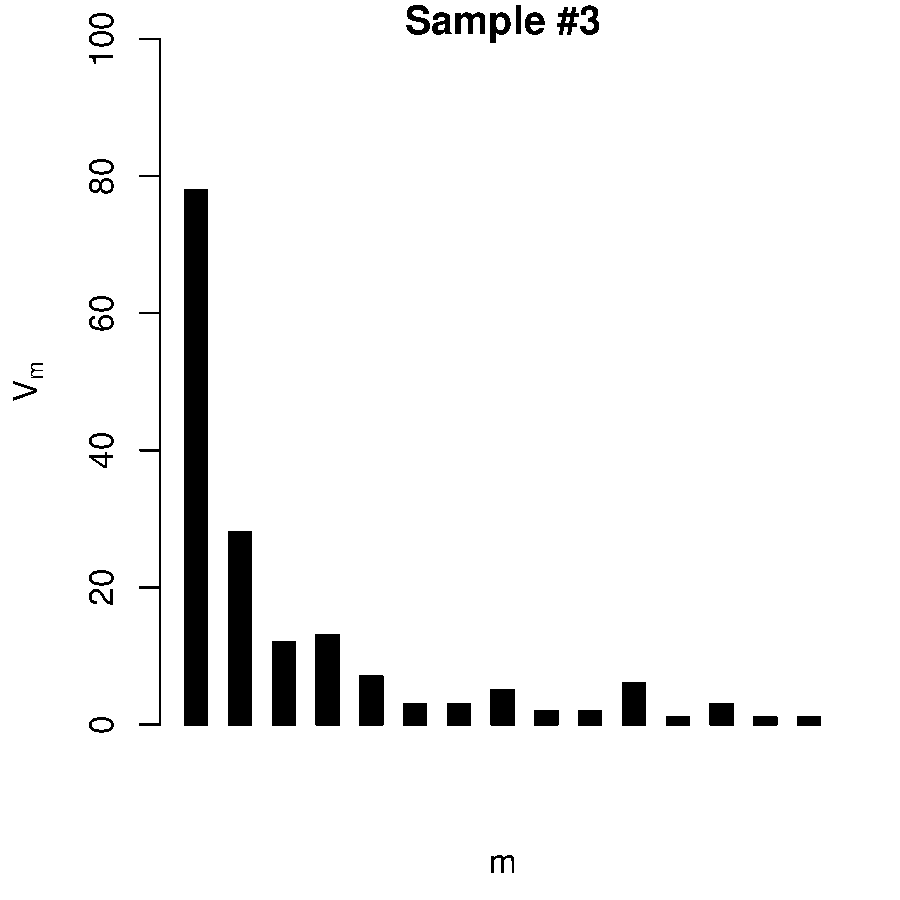
\includegraphics[width=40mm]{img/02-samples-spc-3} &
      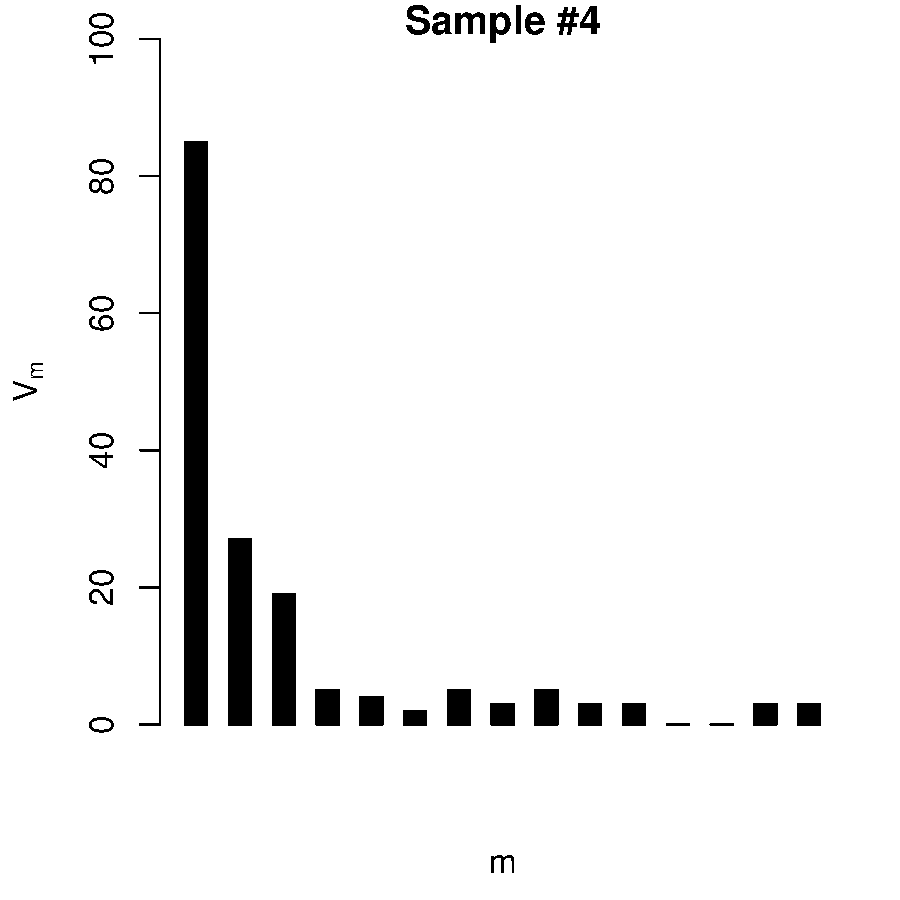
\includegraphics[width=40mm]{img/02-samples-spc-4} 
    \end{tabular}
  \end{center}
\end{frame}

\begin{frame}
  \frametitle{Random variation: vocabulary growth curve}

  \begin{center}
    \begin{tabular}{cc}
      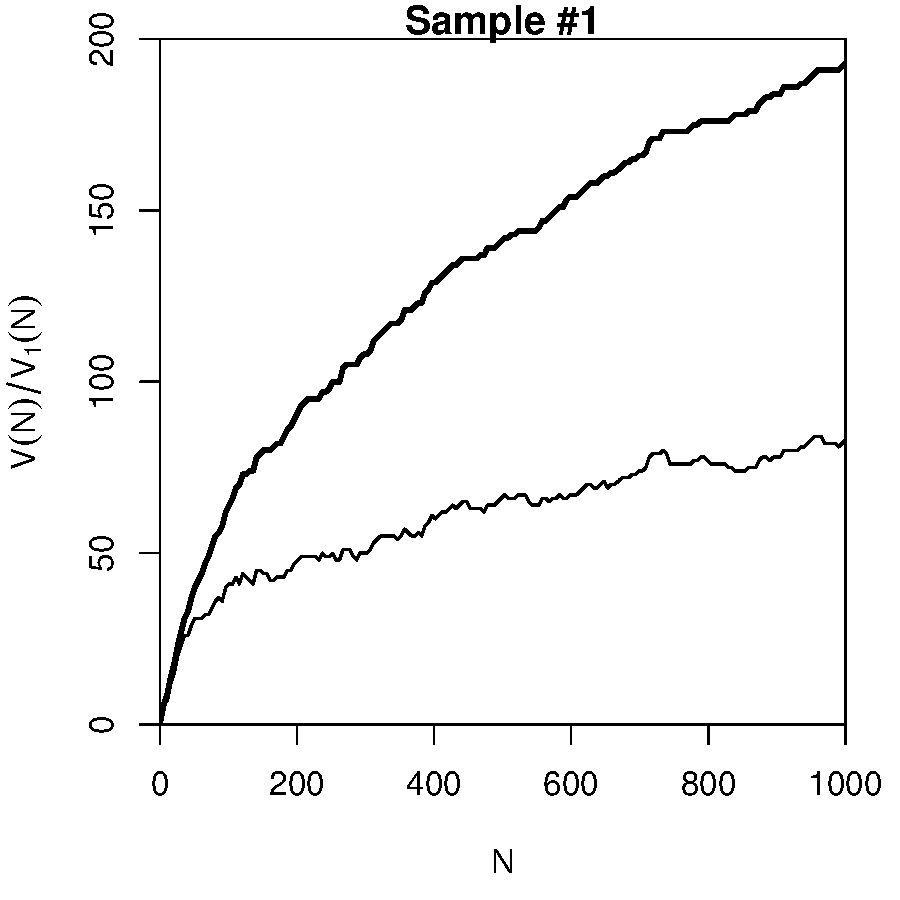
\includegraphics[width=40mm]{img/02-samples-vgc-1} &
      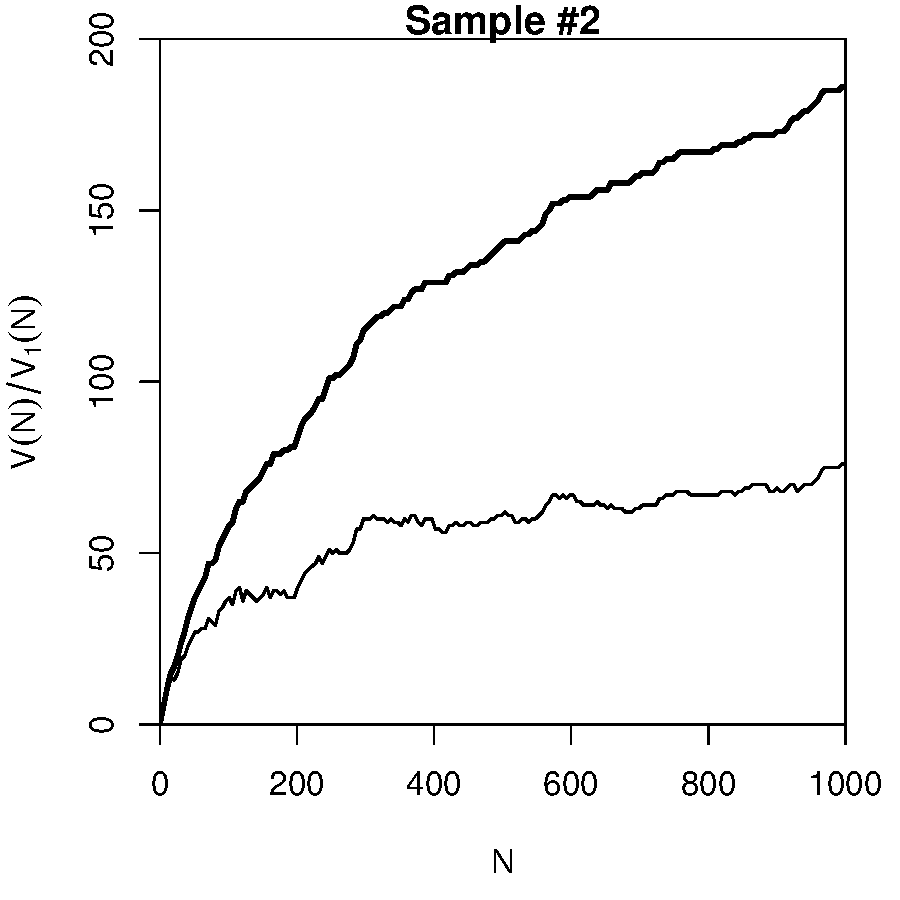
\includegraphics[width=40mm]{img/02-samples-vgc-2} \\
      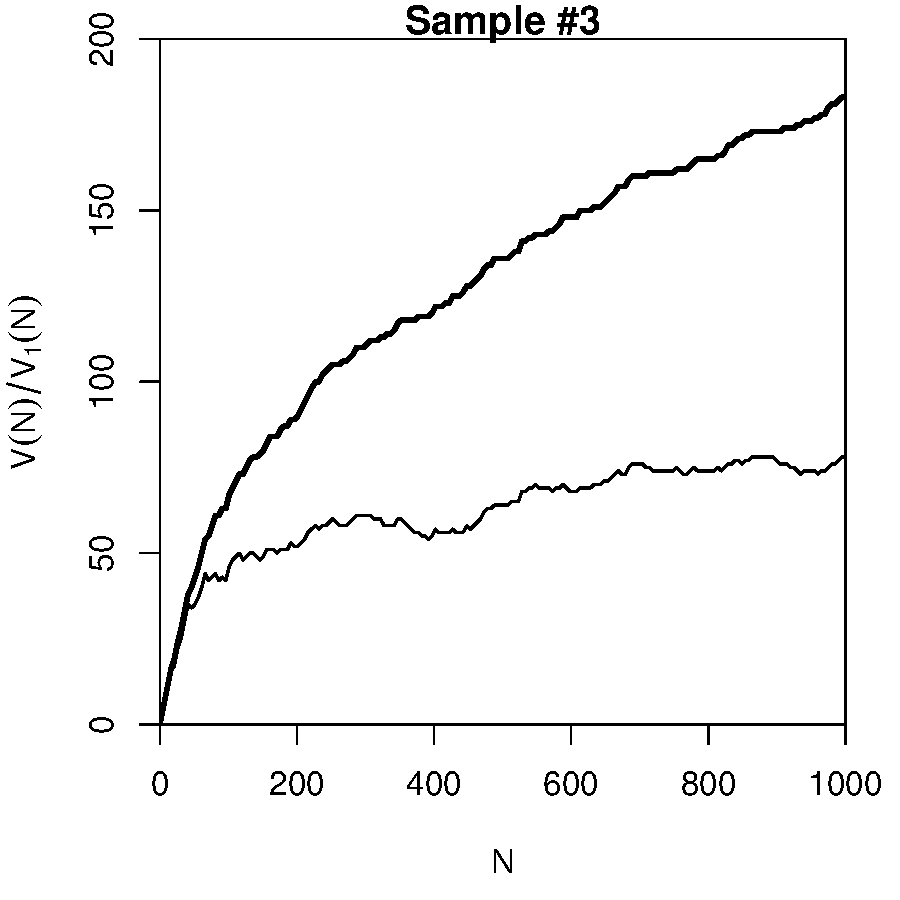
\includegraphics[width=40mm]{img/02-samples-vgc-3} &
      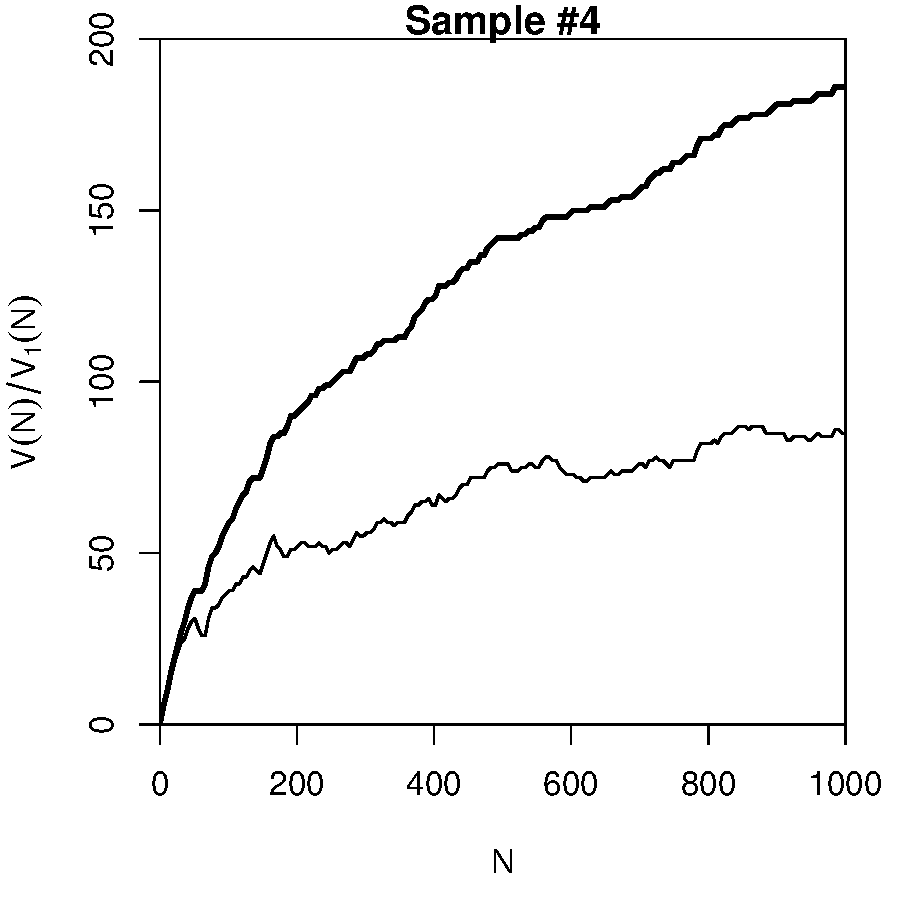
\includegraphics[width=40mm]{img/02-samples-vgc-4} 
    \end{tabular}
  \end{center}
\end{frame}

%%%%%%%%%%%%%%%%%%%%%%%%%%%%%%%%%%%%%%%%%%%%%%%%%%%%%%%%%%%%%%%%%%%%%%%%

\subsection{Great expectations}

\begin{frame}
  \frametitle{Expected values}

  \begin{itemize}
  \item There is no reason why we should choose a particular sample to make a
    prediction for the real data -- each one is equally likely or unlikely
  \item Take the average over a large number of samples, called \h{expected
      value} or \h{expectation} in statistics
  \item[]
  \item Notation: $\text{E}\bigl[V(N)\bigr]$ and $\text{E}\bigl[V_m(N)\bigr]$
    \begin{itemize}
    \item indicates that we are referring to expected values for a sample of
      size $N$
    \item rather than to the specific values $V$ and $V_m$\\
      observed in a particular sample or a real-world data set
    \end{itemize}
  \item[]
  \item Expected values can be calculated efficiently \emph{without}
    generating thousands of random samples
  \end{itemize}
\end{frame}

\begin{frame}
  \frametitle{The expected frequency spectrum}

  \begin{center}
    \begin{tabular}{cc}
      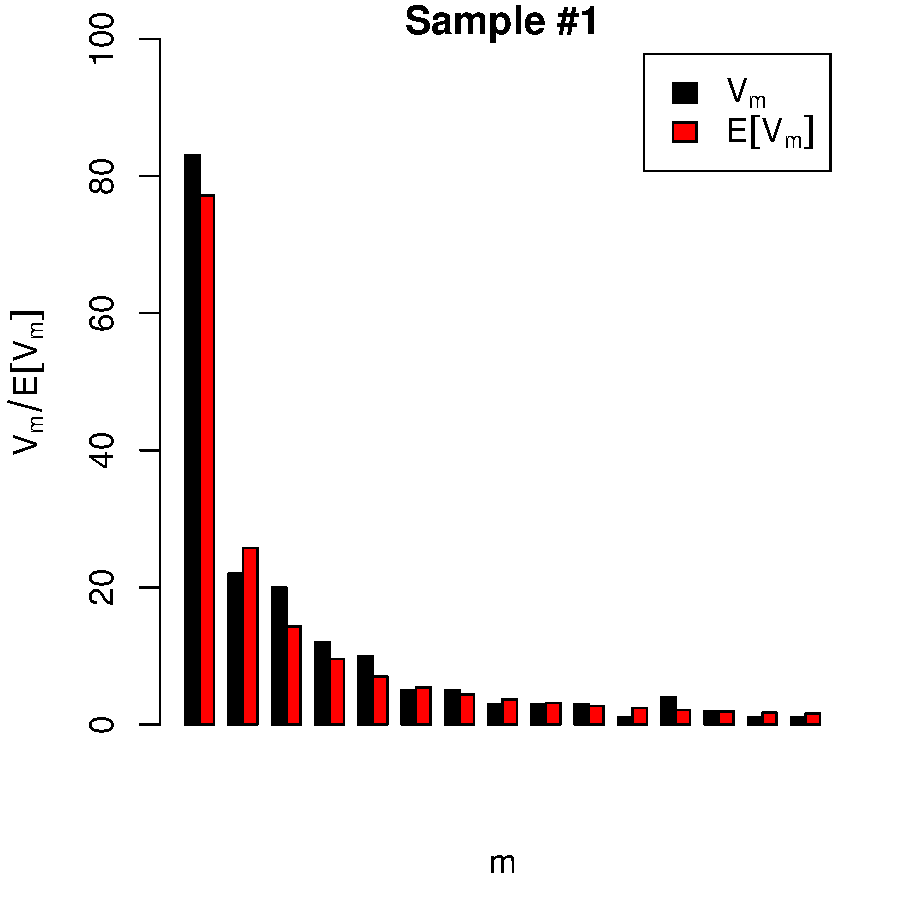
\includegraphics[width=40mm]{img/02-samples-spc-exp-vs-sample-1} &
      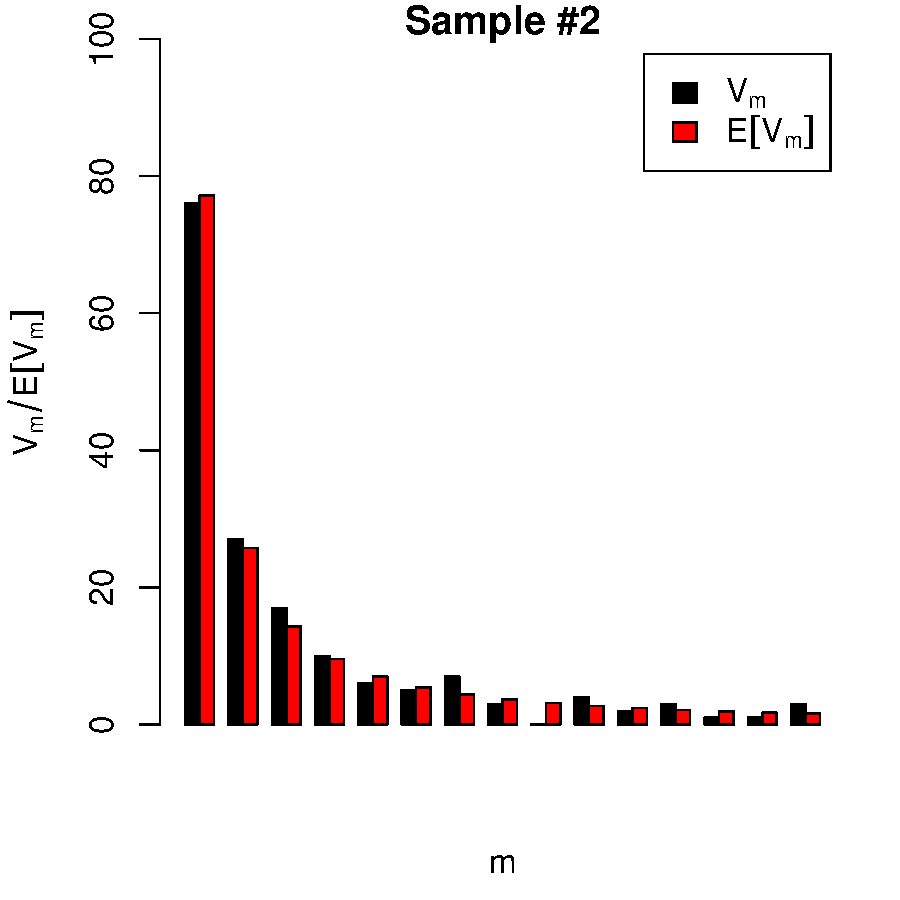
\includegraphics[width=40mm]{img/02-samples-spc-exp-vs-sample-2} \\
      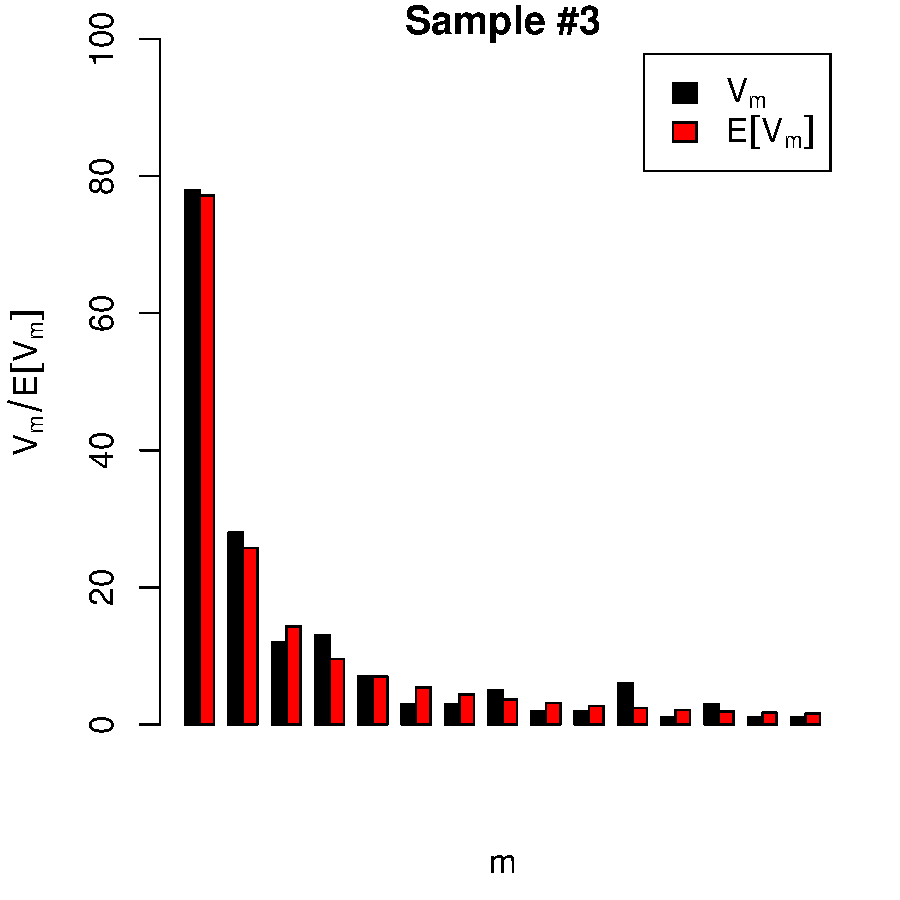
\includegraphics[width=40mm]{img/02-samples-spc-exp-vs-sample-3} &
      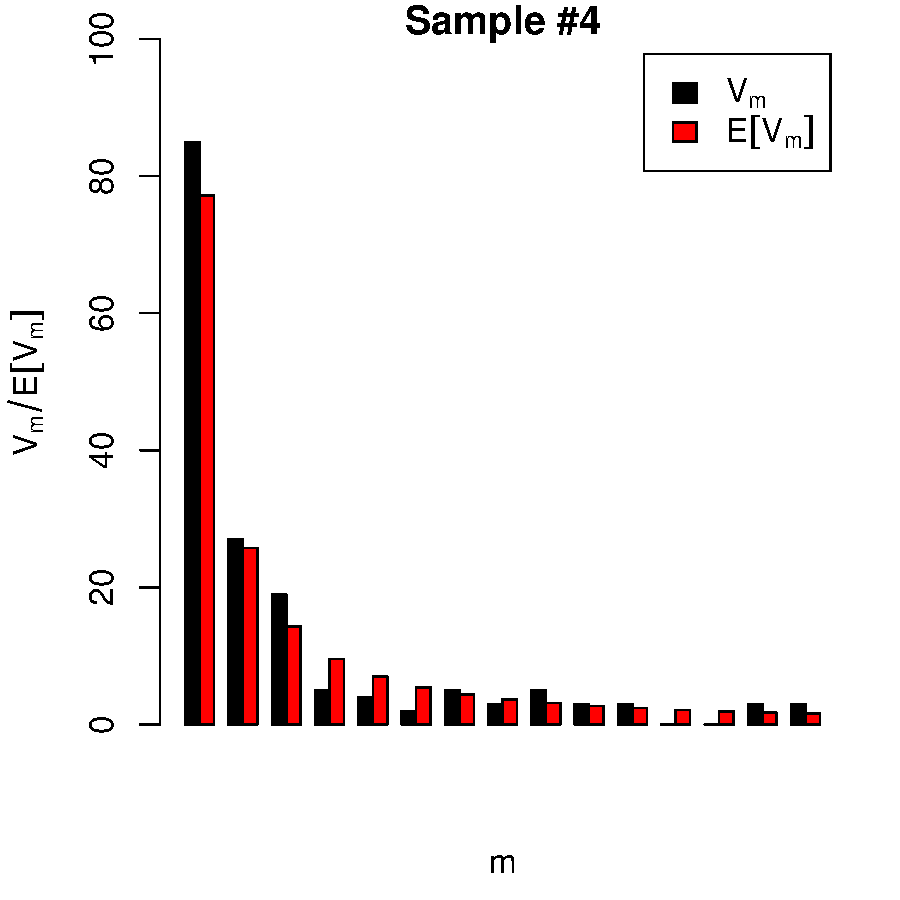
\includegraphics[width=40mm]{img/02-samples-spc-exp-vs-sample-4} 
    \end{tabular}
  \end{center}
\end{frame}

\begin{frame}
  \frametitle{The expected vocabulary growth curve}

  \begin{center}
    \begin{tabular}{c @{} c}
      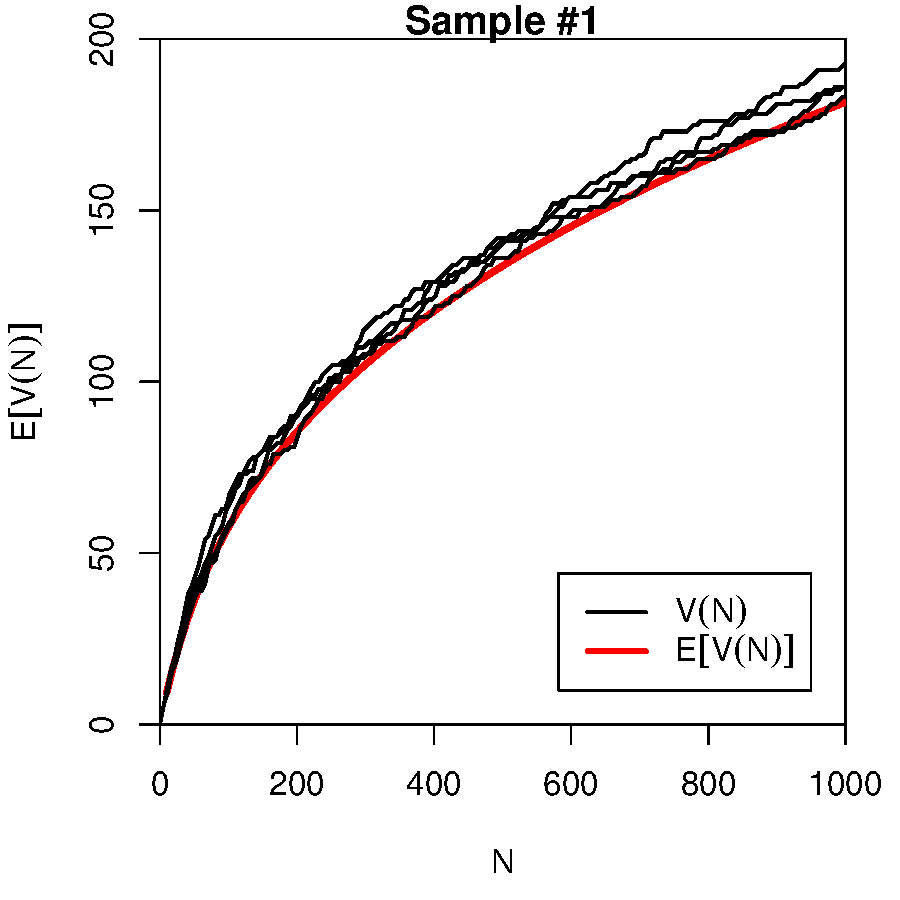
\includegraphics[width=50mm]{img/02-samples-vgc-exp-vs-samples} &
      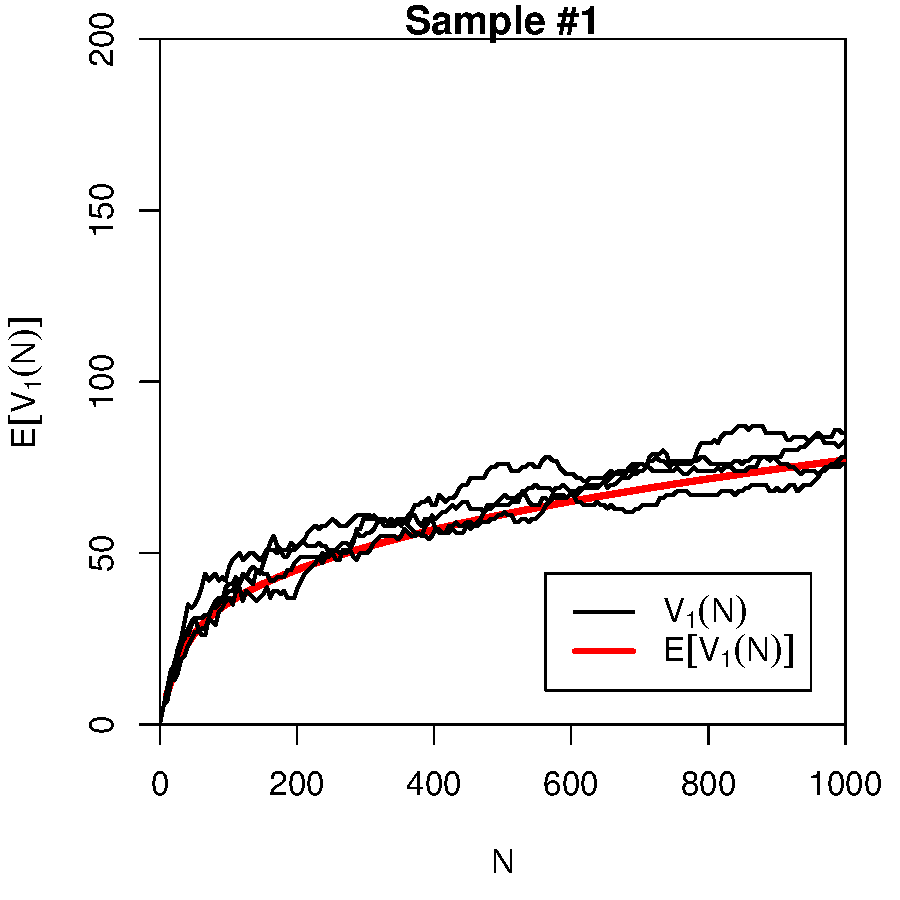
\includegraphics[width=50mm]{img/02-samples-vgc-V1-exp-vs-samples}
    \end{tabular}
  \end{center}
\end{frame}

\begin{frame}
  \frametitle{Confidence intervals for the expected VGC}

  \begin{center}
    \begin{tabular}{c @{} c}
      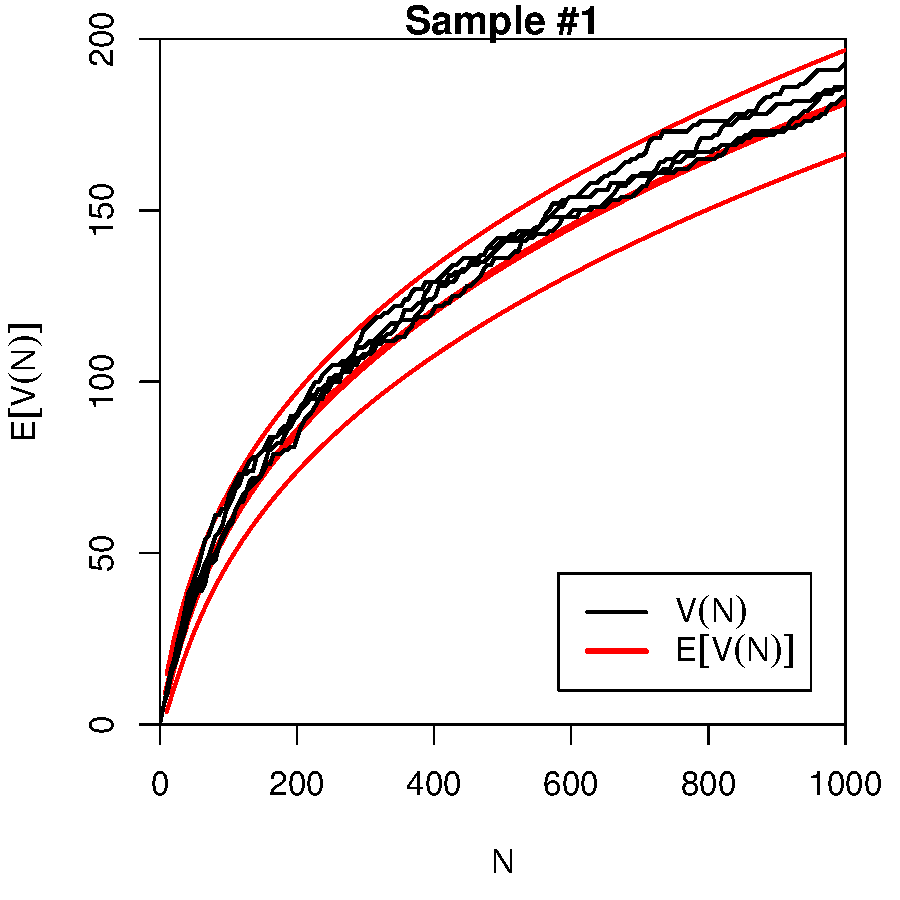
\includegraphics[width=50mm]{img/02-samples-vgc-exp-vs-samples-conf} &
      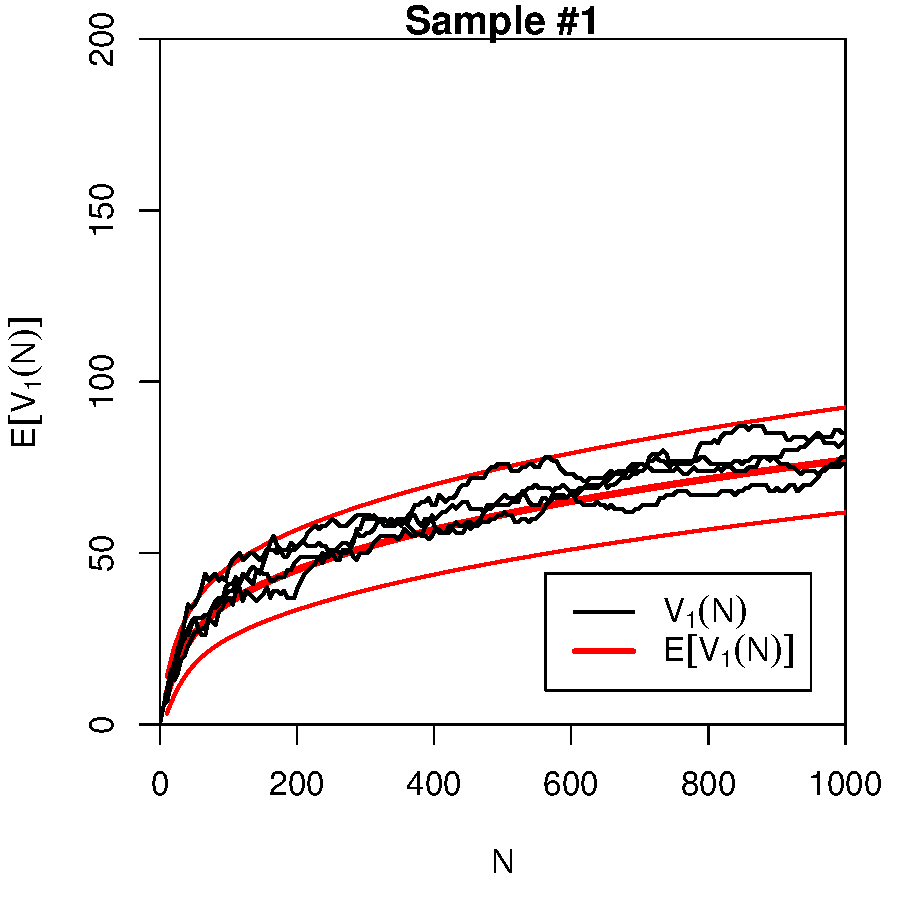
\includegraphics[width=50mm]{img/02-samples-vgc-V1-exp-vs-samples-conf}
    \end{tabular}
  \end{center}
\end{frame}

%%%%%%%%%%%%%%%%%%%%%%%%%%%%%%%%%%%%%%%%%%%%%%%%%%%%%%%%%%%%%%%%%%%%%%%%

\subsection{Parameter estimation for LNRE models }

\begin{frame}<beamer:1-7| handout:1-3,7>
  \frametitle{Parameter estimation by trial \& error}

  \begin{center}
    \begin{tabular}{c @{} c}
      \only<beamer:1| handout:1>{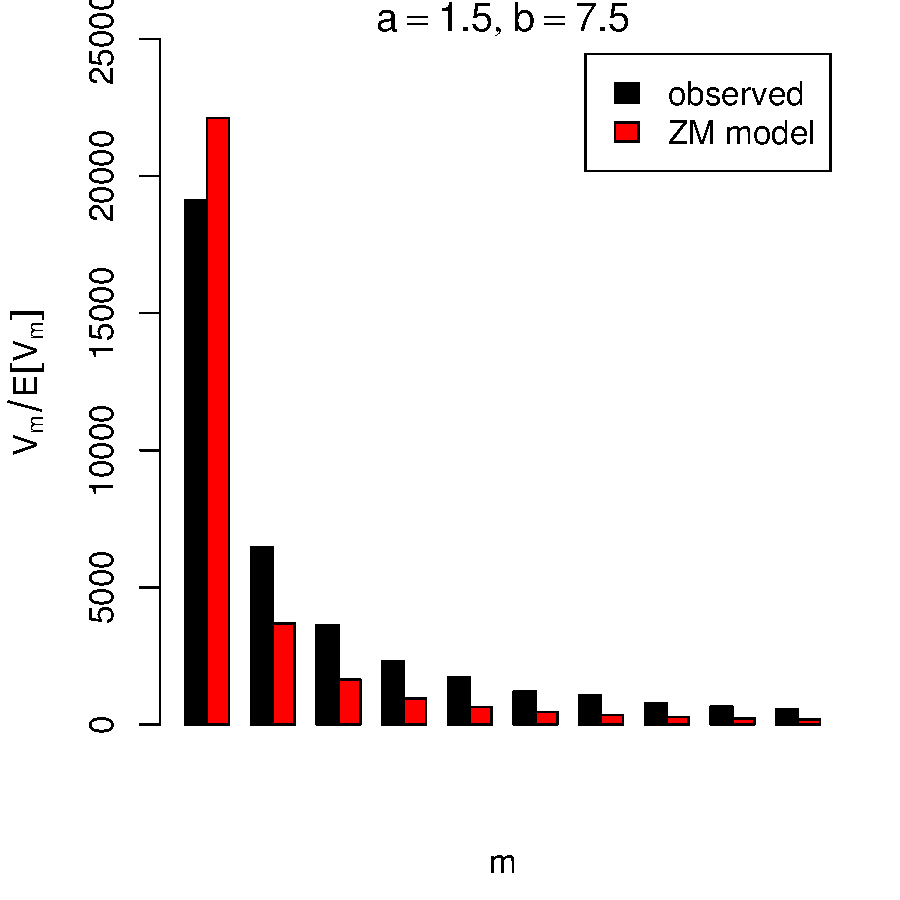
\includegraphics[width=50mm]{img/02-estimation-spc-1}}%
      \only<beamer:2| handout:2>{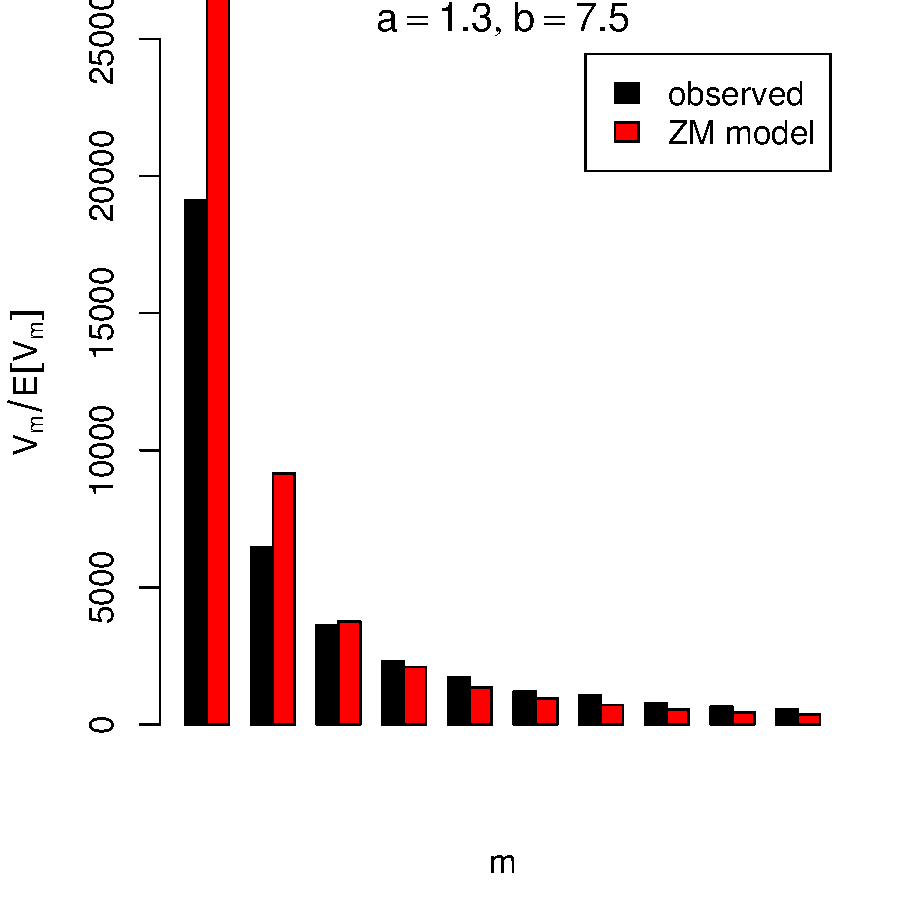
\includegraphics[width=50mm]{img/02-estimation-spc-2}}%
      \only<beamer:3| handout:3>{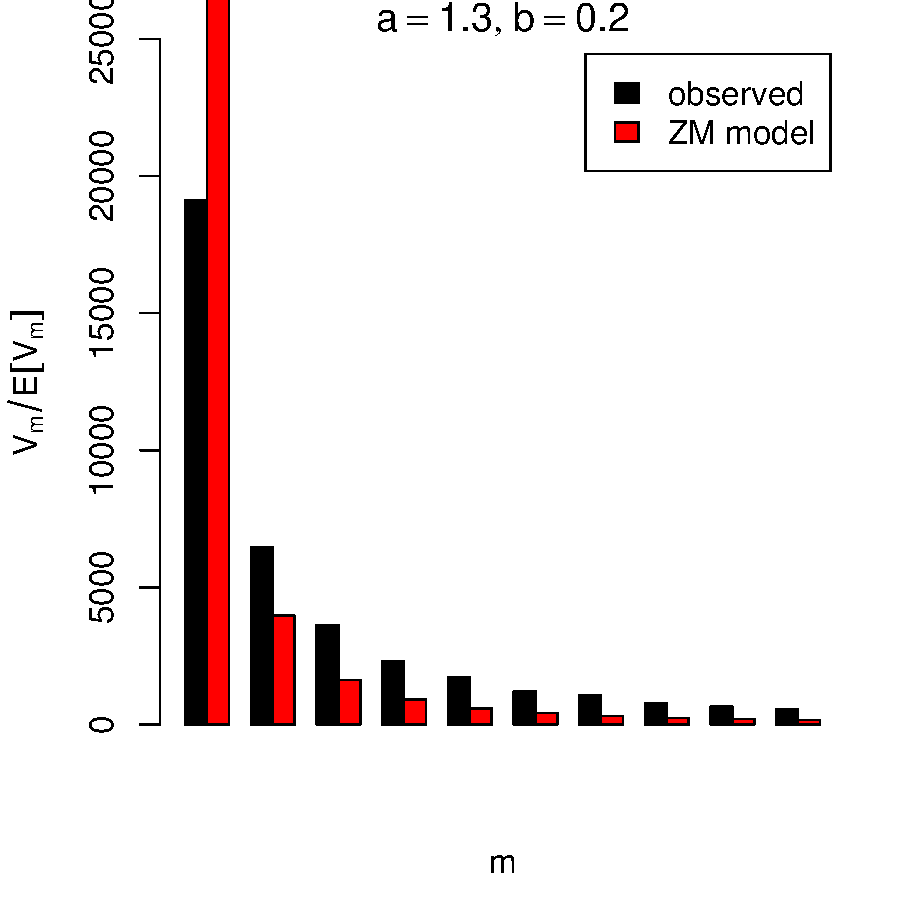
\includegraphics[width=50mm]{img/02-estimation-spc-3}}%
      \only<beamer:4| handout:0>{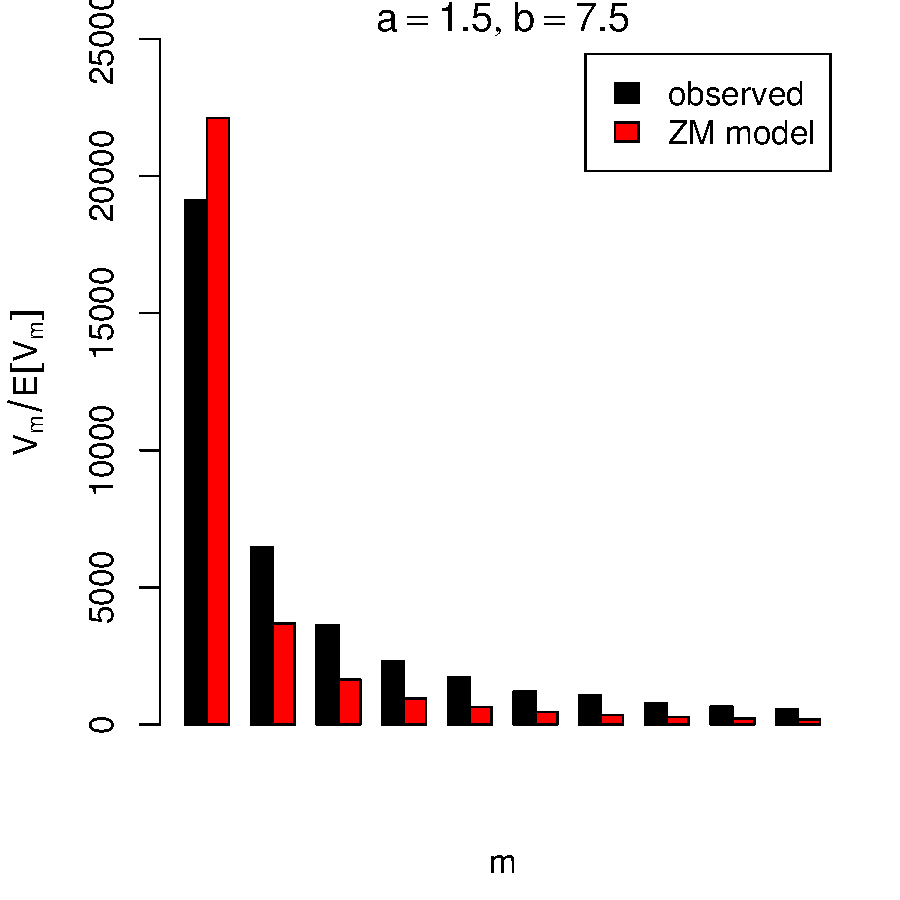
\includegraphics[width=50mm]{img/02-estimation-spc-1}}%
      \only<beamer:5| handout:0>{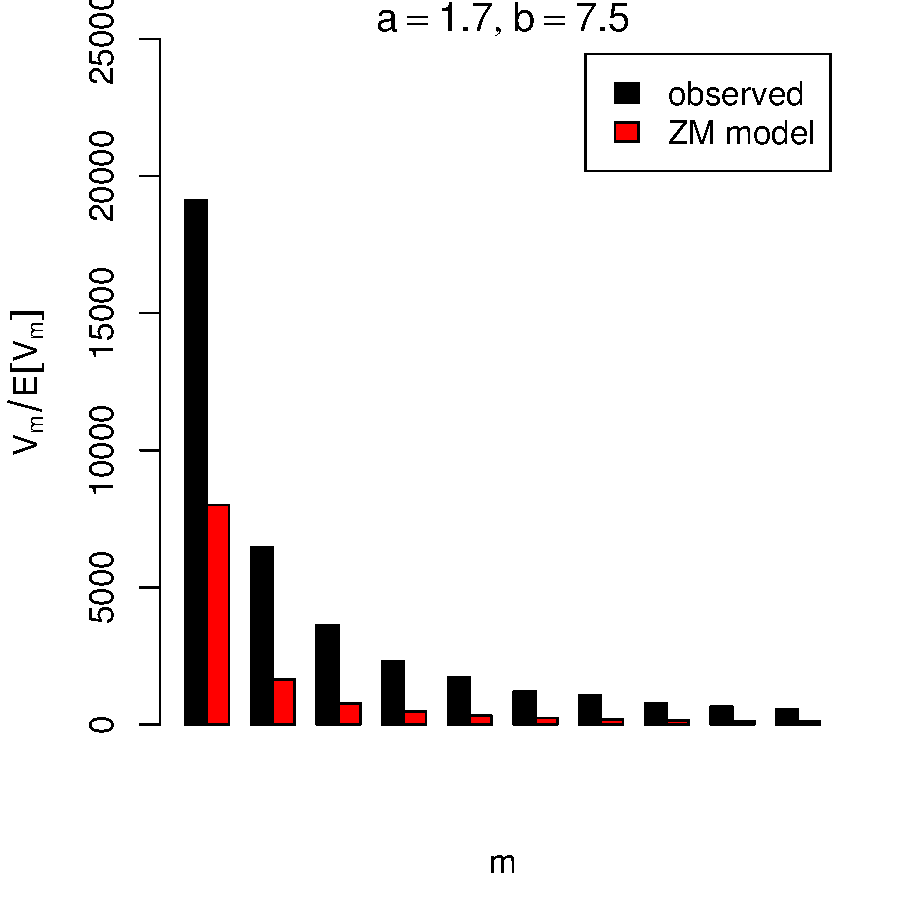
\includegraphics[width=50mm]{img/02-estimation-spc-4}}%
      \only<beamer:6| handout:0>{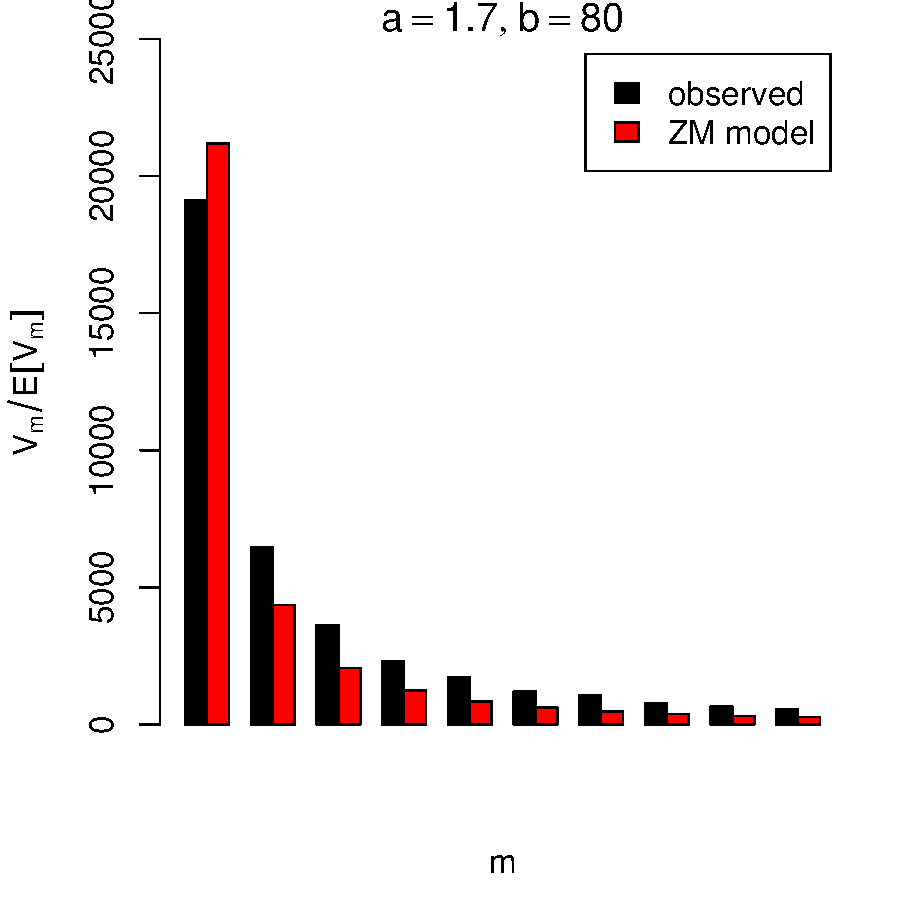
\includegraphics[width=50mm]{img/02-estimation-spc-5}}%
      \only<beamer:7| handout:7>{\includegraphics[width=50mm]{img/02-estimation-spc-6}}%
      &
      \only<beamer:1| handout:1>{\includegraphics[width=50mm]{img/02-estimation-vgc-1}}%
      \only<beamer:2| handout:2>{\includegraphics[width=50mm]{img/02-estimation-vgc-2}}%
      \only<beamer:3| handout:3>{\includegraphics[width=50mm]{img/02-estimation-vgc-3}}%
      \only<beamer:4| handout:0>{\includegraphics[width=50mm]{img/02-estimation-vgc-1}}%
      \only<beamer:5| handout:0>{\includegraphics[width=50mm]{img/02-estimation-vgc-4}}%
      \only<beamer:6| handout:0>{\includegraphics[width=50mm]{img/02-estimation-vgc-5}}%
      \only<beamer:7| handout:7>{\includegraphics[width=50mm]{img/02-estimation-vgc-6}}%
    \end{tabular}
  \end{center}
\end{frame}

\begin{frame}
  \frametitle{Automatic parameter estimation}
  \framesubtitle{Minimisation of suitable cost function for frequency spectrum}

  \begin{center}
    \begin{tabular}{c @{} c}
      \includegraphics[width=50mm]{img/02-estimation-spc-estimated} &
      \includegraphics[width=50mm]{img/02-estimation-vgc-estimated} 
    \end{tabular}
  \end{center}

  \begin{itemize}
    \item By trial \& error we found $a=2.0$ and $b=550$
    \item Automatic estimation procedure: $a=2.39$ and $b=1968$
    \item Goodness-of-fit: $p\approx 0$ (multivariate chi-squared test)
  \end{itemize}
\end{frame}

\begin{frame}
  \frametitle{Summary}

  LNRE modelling in a nutshell:%
  \pause
  \begin{enumerate}
  \item compile \h{observed} frequency spectrum (and vocabulary growth curves)
    for a given corpus or data set%
    \pause
  \item estimate parameters of \h{LNRE model} by matching observed and
    expected frequency spectrum%
    \pause
  \item evaluate \h{goodness-of-fit} on spectrum (Baayen 2001) or by
    testing extrapolation accuracy (Baroni \& Evert 2007)
    \begin{itemize}
      \item in principle, you should only go on if model gives a plausible
        explanation of the observed data!
    \end{itemize}
    \pause
  \item use LNRE model to compute \h{expected} frequency spectrum for
    arbitrary sample sizes\\
    \so \h{extrapolation} of vocabulary growth curve
    \begin{itemize}
    \item or use population model directly as Bayesian prior etc.
    \end{itemize}
  \end{enumerate}
\end{frame}

%%%%%%%%%%%%%%%%%%%%%%%%%%%%%%%%%%%%%%%%%%%%%%%%%%%%%%%%%%%%%%%%%%%%%%%%

\section{zipfR}

\begin{frame}
  \frametitle{zipfR}

  \begin{itemize}
  \item \url{http://purl.org/stefan.evert/zipfR}
  \item Conveniently available from CRAN repository
  \item Explore your GUI for general package installation and management
    options
  \end{itemize}

  \vspace{-6mm}
  \begin{flushright}
    \includegraphics[width=6cm]{img/zipfR_logo}
    \rule{1cm}{0mm}
  \end{flushright}

\end{frame}

\begin{frame}[fragile]
  \frametitle{Loading}

\begin{verbatim}
> library(zipfR)

> ?zipfR

> data(package="zipfR")
\end{verbatim}

\end{frame}


\begin{frame}[fragile]
  \frametitle{Importing data}

\begin{verbatim}
> data(ItaRi.spc)
> data(ItaRi.emp.vgc)

> my.spc <- read.spc("my.spc.txt")
> my.vgc <- read.vgc("my.vgc.txt")

> my.tfl <- read.tfl("my.tfl.txt")
> my.spc <- tfl2spc(my.tfl)
\end{verbatim}

\end{frame}

\begin{frame}[fragile]
  \frametitle{Looking at spectra}

\begin{alltt}
> summary(ItaRi.spc)
> ItaRi.spc

> N(ItaRi.spc)
> V(ItaRi.spc)
> Vm(ItaRi.spc,1)
> Vm(ItaRi.spc,1:5)

\REM{Baayen's P}
> Vm(ItaRi.spc,1) / N(ItaRi.spc)

> plot(ItaRi.spc)
> plot(ItaRi.spc, log="x")
\end{alltt}
\end{frame}

\begin{frame}[fragile]
  \frametitle{Looking at VGCs}

\begin{verbatim}
> summary(ItaRi.emp.vgc)
> ItaRi.emp.vgc

> N(ItaRi.emp.vgc)

> plot(ItaRi.emp.vgc, add.m=1)
\end{verbatim}
\end{frame}

\begin{frame}[fragile]
  \frametitle{Creating VGCs with binomial interpolation}

\begin{alltt}
\REM{interpolated VGC}

> ItaRi.bin.vgc <- vgc.interp(ItaRi.spc,
  N(ItaRi.emp.vgc), m.max=1)

> summary(ItaRi.bin.vgc)

\REM{comparison}

> plot(ItaRi.emp.vgc, ItaRi.bin.vgc,
  legend=c("observed","interpolated"))
\end{alltt}


\end{frame}


\begin{frame}
  \frametitle{\emph{ultra-}}

  \begin{itemize}
  \item Load the spectrum and empirical VGC of the less common prefix \emph{ultra-}
  \item Compute binomially interpolated VGC for \emph{ultra-}
  \item Plot the binomially interpolated \emph{ri-} and \emph{ultra-}
    VGCs together
  \end{itemize}

\end{frame}


\begin{frame}[fragile]
  \frametitle{Estimating LNRE models}

\begin{alltt}
\REM{fZM model; you can also try ZM and GIGP, and compare}

> ItaUltra.fzm <- lnre("fzm", ItaUltra.spc)

> summary(ItaUltra.fzm)
\end{alltt}

\end{frame}


\begin{frame}[fragile]
  \frametitle{Observed/expected spectra at estimation size}
\begin{alltt}
\REM{expected spectrum}

> ItaUltra.fzm.spc <- lnre.spc(ItaUltra.fzm, 
  N(ItaUltra.fzm))

\REM{compare}

> plot(ItaUltra.spc, ItaUltra.fzm.spc,
  legend=c("observed","fzm"))

\REM{plot first 10 elements only}

> plot(ItaUltra.spc, ItaUltra.fzm.spc, 
  legend=c("observed","fzm"), m.max=10)
\end{alltt}
\end{frame}

% \begin{frame}[fragile]
%   \frametitle{Expected spectra at 10 times the estimation size}
% \begin{alltt}
% \REM{extrapolated spectra}

% ItaRi.zm.spc <- lnre.spc(ItaRi.zm, 10*N(ItaRi.zm))

% ItaRi.fzm.spc <- lnre.spc(ItaRi.fzm, 
% 10*N(ItaRi.fzm))

% \REM{compare}

% plot(ItaRi.zm.spc, ItaRi.fzm.spc,
% legend=c("zm","fzm"))
% \end{alltt}
% \end{frame}

% \begin{frame}[fragile]
%   \frametitle{Evaluating extrapolation quality 1}

% \begin{alltt}
% \REM{taking a subsample and estimating a model (if you
% # repat you'll get different sample and different 
% # model!)}

% ItaRi.sub.spc <- sample.spc(ItaRi.spc, N=700000)

% ItaRi.sub.fzm <- lnre("fzm", ItaRi.sub.spc)

% ItaRi.sub.fzm
% \end{alltt}
% \end{frame}


% \begin{frame}[fragile]
%   \frametitle{Evaluating extrapolation quality 2}

% \begin{alltt}
% \REM{extrapolate vgc up to original sample size}

% ItaRi.sub.fzm.vgc <- lnre.vgc(ItaRi.sub.fzm, 
% N(ItaRi.emp.vgc))

% \REM{compare}

% plot(ItaRi.bin.vgc, ItaRi.sub.fzm.vgc,
% N0=N(ItaRi.sub.fzm), legend=c("interpolated","fZM"))
% \end{alltt}
% \end{frame}


% \begin{frame}[fragile]
%   \frametitle{Compare growth of two categories 1}
% \begin{alltt}
% \REM{the ultra- prefix}

% data(ItaUltra.spc)

% summary(ItaUltra.spc)

% \REM{cf.}

% summary(ItaRi.spc)

% \REM{estimating model}

% ItaUltra.fzm <- lnre("fzm",ItaUltra.spc,exact=F)

% ItaUltra.fzm

% \end{alltt}
% \end{frame}


\begin{frame}[fragile]
  \frametitle{Compare growth of two categories}
\begin{alltt}
\REM{extrapolation of \emph{ultra-} VGC to sample size of \emph{ri-} data}

> ItaUltra.ext.vgc <- lnre.vgc(ItaUltra.fzm,
  N(ItaRi.emp.vgc))

\REM{compare}

> plot(ItaUltra.ext.vgc, ItaRi.bin.vgc,
  N0=N(ItaUltra.fzm), legend=c("ultra-","ri-"))

\REM{zooming in}

> plot(ItaUltra.ext.vgc, ItaRi.bin.vgc,
  N0=N(ItaUltra.fzm), legend=c("ultra-","ri-"),
  xlim=c(0,1e+5))
\end{alltt}
\end{frame}

\end{document}
